%!TEX root = ../report.tex

\begin{document}
    \chapter{Experimental Setup}
    \label{chap:experiment_setup}
    \section{Libraries and Toolkits}
    
    In order to do seamless experiments, a lot of libraries and toolkits came in handy while parsing, preprocessing the text, and extracting the features. These libraries include functions which would do the most repetitive tasks in NLP that would require significant time to code from scratch. The open source libraries which were used in our experiments include Numpy, Pandas, NLTK, Spacy, and scikit-learn. These are discussed below.
    
    \subsection{Numpy}
    
    Numpy is a handy library in Python which is used to work with multidimensional arrays and matrices along with some high-level mathematical functions to operate on these arrays. In addition, it has functions with linear algebra, Fourier transform, and random number capabilities \cite{numpy}.
    
    \subsection{Pandas}
    
    Pandas provides high-end, easy-to-use data structure and data analysis tools written in Python programming language \cite{pandas}. It was helpful in filtering out the required fields from the dataset and visualize the results of preprocessing steps in a structured manner.  
    
    \subsection{NLTK - Natural Language Toolkit}
    
    Natural Language Toolkit is a platform for working on human language using Python. It is open-source and one of the most versatile libraries available today. It has a collection of huge corpora and a large set of lexical database. In addition, it has functionalities for various NLP tasks including classification, tokenization, stemming, tagging, parsing, and semantic reasoning \cite{nltk}.
    
    \subsection{spaCy}
    
    spaCy is a very famous open-source libary which is extensively used in various applications of Natural Language Processing written in the programming languages such as Python and Cython. It is more suitable for large-scale information extraction tasks as it is fast and efficient, with seamless interoperation with most of the deep learning libraries and frameworks. Non-destructive tokenization, Named entity recognition, support for 31+ languages, 13 statistical models for 8 languages, Pre-trained word vectors, and Part-of-speech tagging are some of its features. Opposed to NLTK, which is widely used for teaching and research, spaCy is focused more on providing software for production usage \cite{spacy}.
    
    \subsection{ModAL}
    
    ModAL \cite{modAL2018} is a Python3 based framework for active learning which acts as a wrapper over scikit-learn library. It allows easy incorporating of active learning query strategies such as uncertainty based ones and committee based sampling with other functionalities to change the batch size. In addition, it allows to write custom query strategies which was used to perform random sampling in the experiments in this project. 
    
    \subsection{scikit-learn}
    
    scikit-learn is widely used for data mining and data analysis tasks as it is very efficient and simple to use. It is built over Scipy, Numpy and matplotlib. It is an open-source library written in Python programming language. The most prominent algorithms built in this library include classification, regression, clustering, dimensionality reduction, model selection, and preprocessing. We used scikit-learn to employ different machine learning algorithms which would suit best for our task such as logistic regression, naive Bayes classification, and random forest \cite{scikit_learn}. 
    
    
    \section{Datasets}
    
    \subsection{Mohler'11 Dataset}
    
    This dataset was created at the University of North Texas by Rada Mihalcea and Michael Mohler. It consists of the answers for assignments and exams written by undergraduate students of the Computer Science course. The answers were for 10 assignments consisting of 4 to 7 questions each and 2 exams consisting of 10 questions each. The assignments were graded in the range of 0 to 5 whereas the exams were graded from 0 to 10. The exam grades were normalized to 0 to 5 scale for the purpose of using autograding algorithms on them. In total, there were 2273 answers after removing the answers of the questions which were not short-answer type questions and were of selection/ordering type. One of such questions which was removed is "Order the following functions by their running time. $ n^2,  ~log(log(n)), ~n!, ~n^3$". Fig \ref{mohlergrades} shows the grade distribution of all the answers. From this figure, we can clearly determine that the grade distribution is skewed towards the higher grades \cite{Mohler2011}. 
    
    \begin{figure}[h]
    	\centering
    	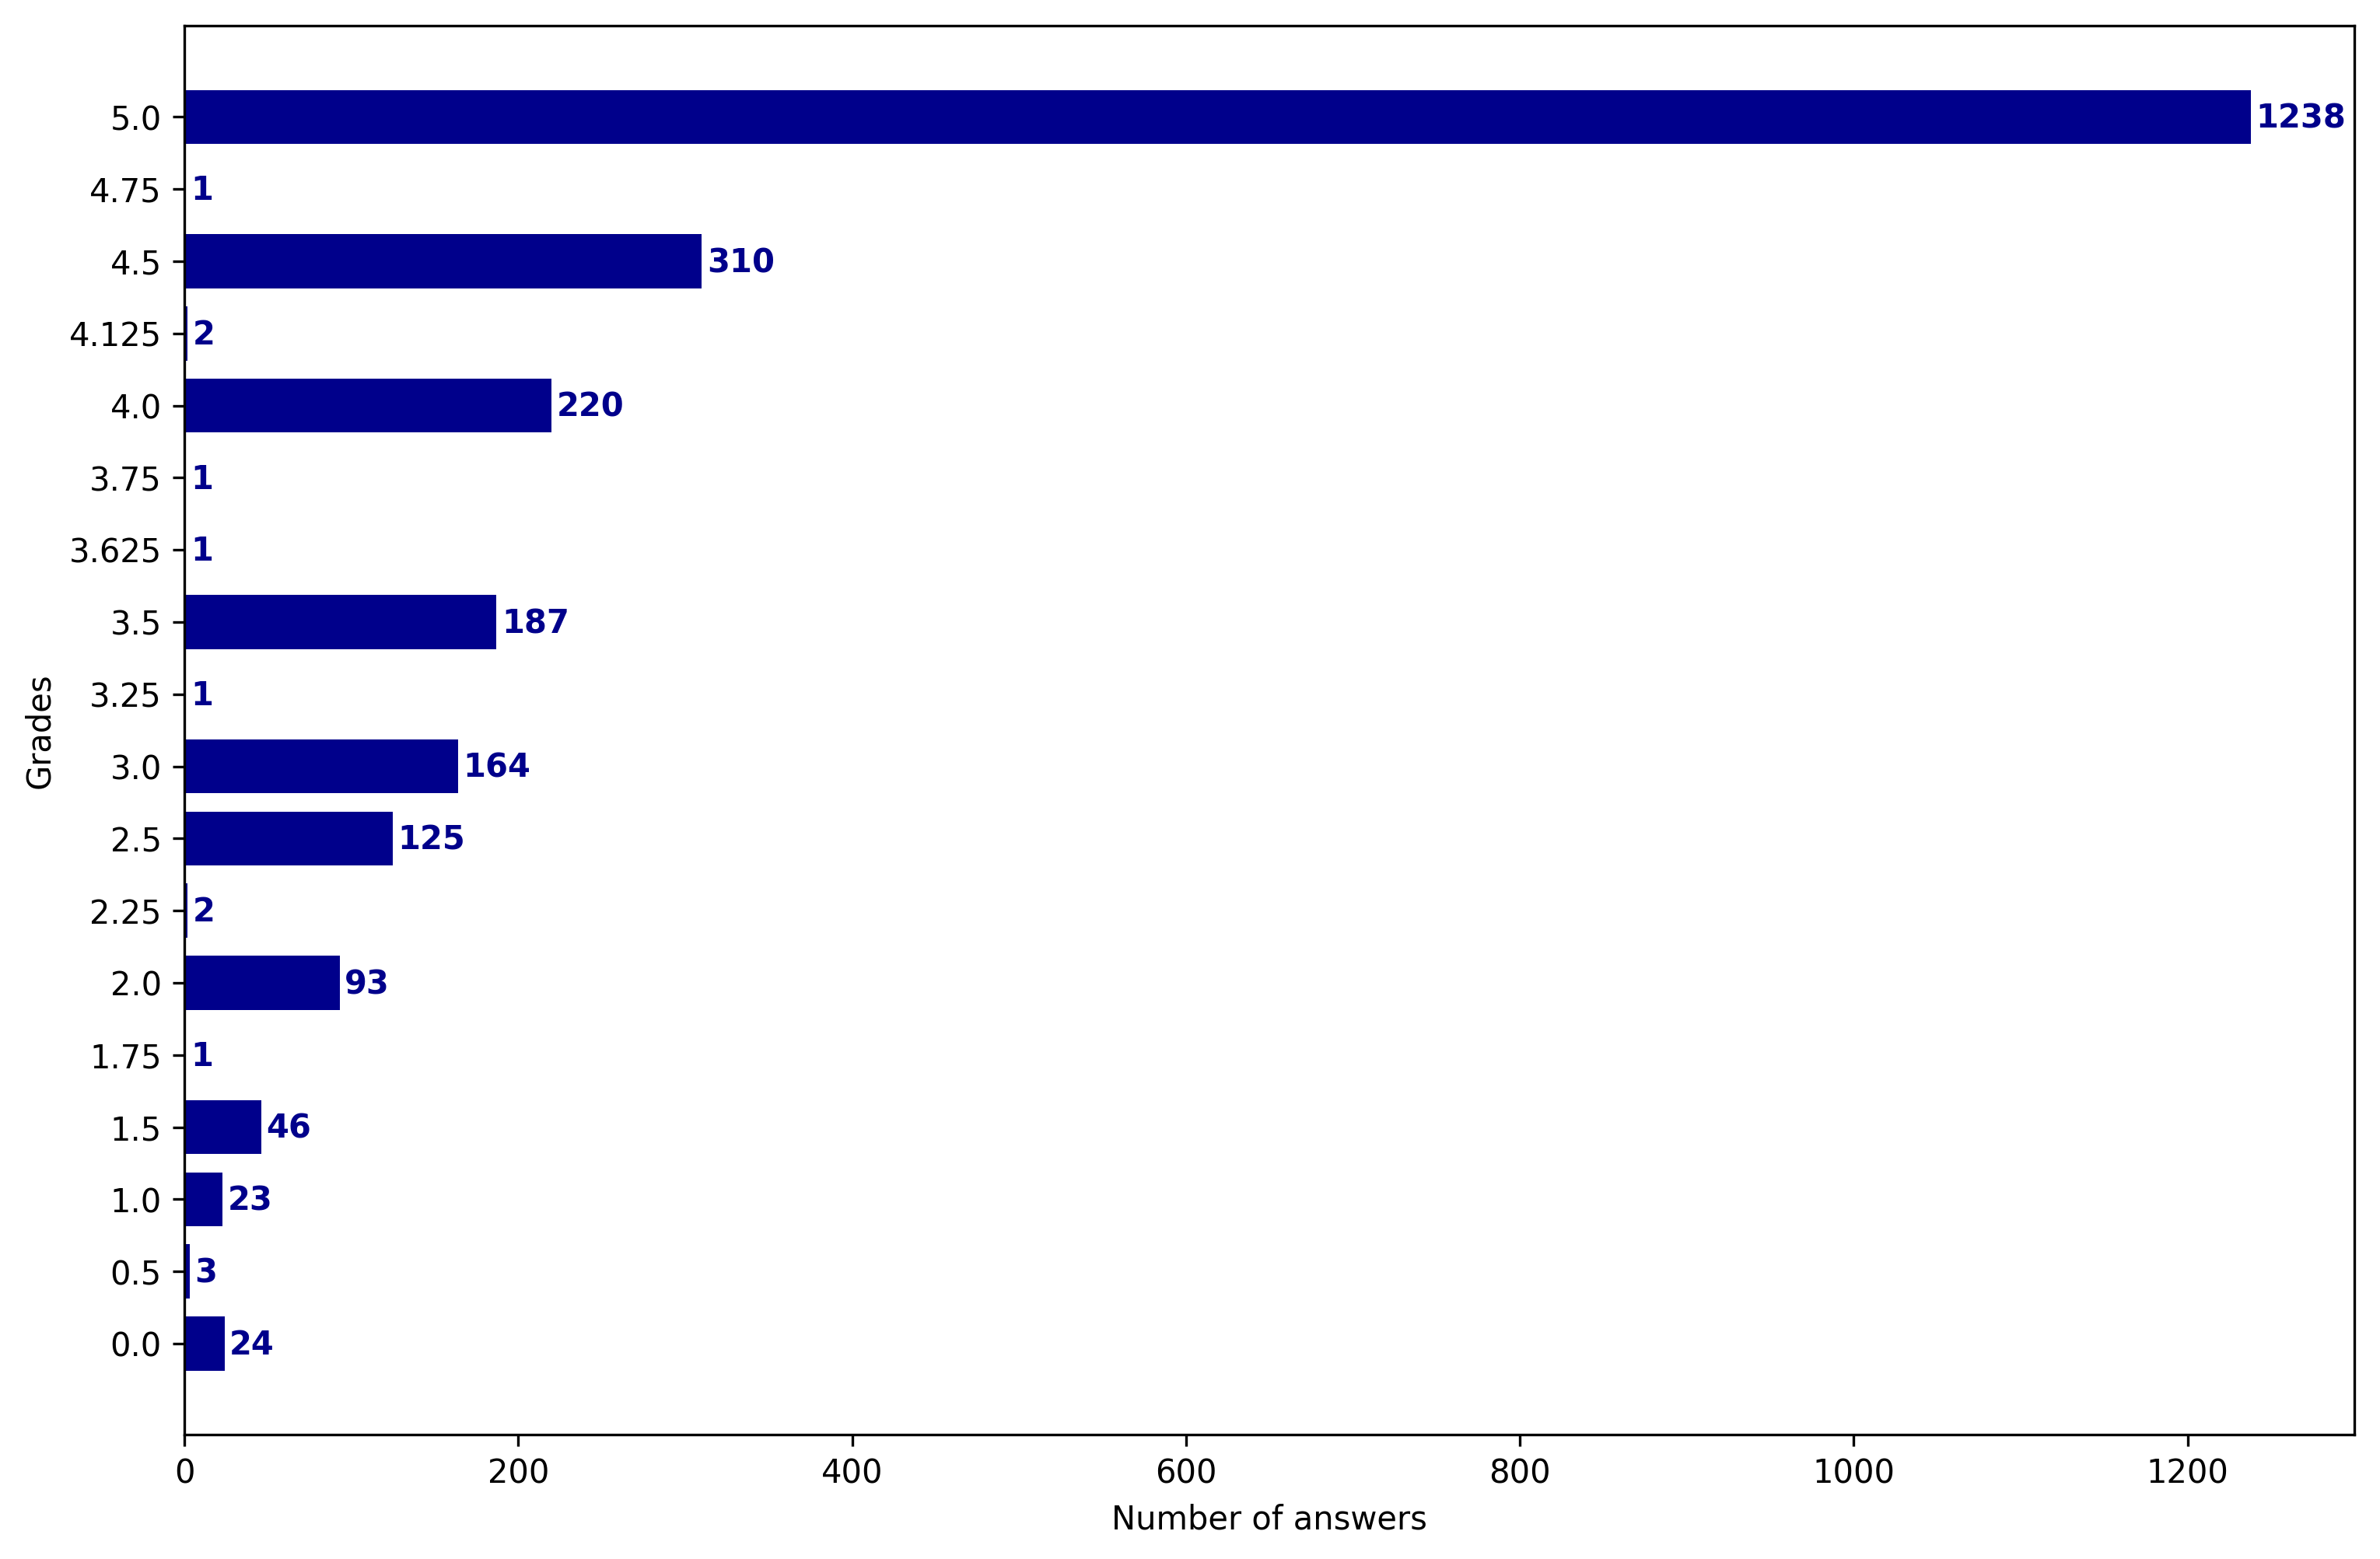
\includegraphics[scale=0.4]{images/mohlergrades}
    	\caption{Grade distribution of Mohler'11 dataset}
	    \label{mohlergrades}
	\end{figure}

	The grades for each answer were given by two graders, and the average of them was provided too. Thus, there were three grades for each and every answer. The average score was used as the ground truth for the experiments conducted with this dataset. The analysis on the grades given by the two annotators revealed that there is a significant percent of disagreement between them. This is illustrated in Fig \ref{mohlerdisagreement}.      

	The Fig \ref{mohlerdisagreement} shows the percentage of answers with respect to the difference in the grades given by each annotator. For e.g., the percentage of answers which were graded by the two annotators with a difference of 3 is 5.5\%. Only 57.7\% of the answers were given the same grades \cite{Mohler2011}.  

	\begin{figure}[h]
		\centering
		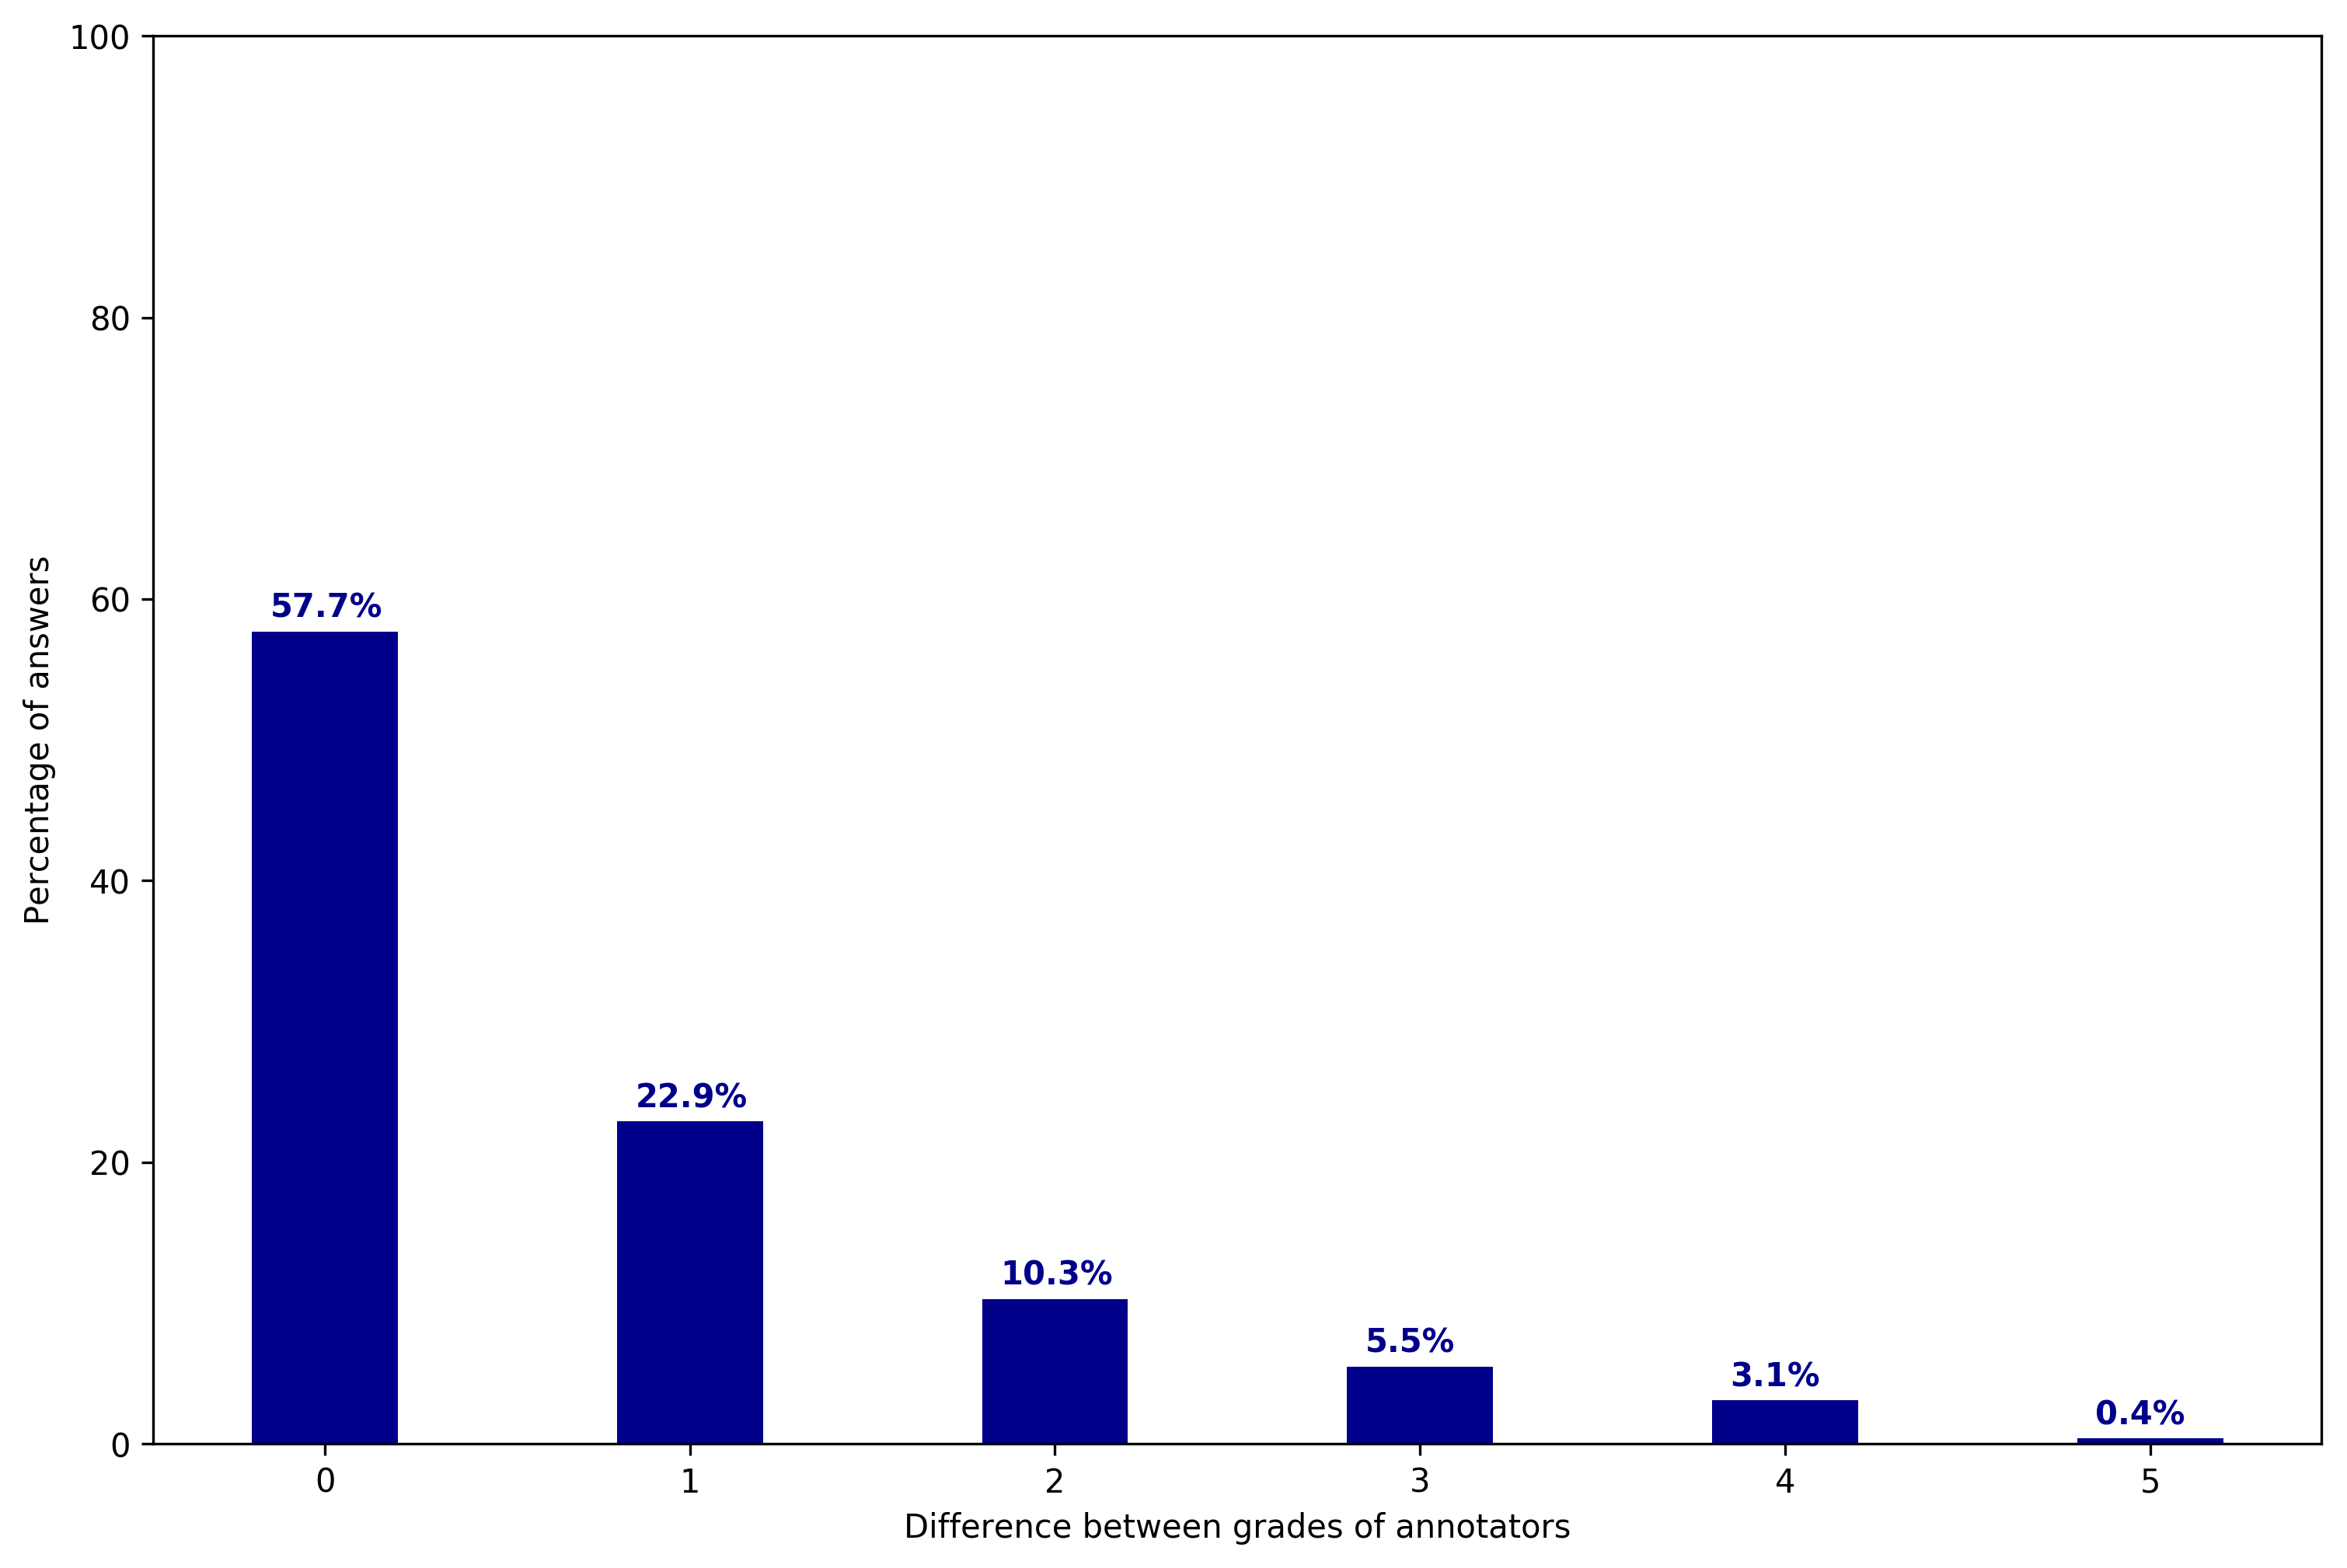
\includegraphics[scale=0.3]{images/mohlerdisagreement}
		\caption{Inter-annotator grade analysis \cite{Mohler2011}}
		\label{mohlerdisagreement}
	\end{figure}
	
	This dataset is chosen for the experiments in this project as it is relatively a big dataset in the ASAG research community. This dataset is often used to benchmark many short answer grading systems such as \cite{Sultan2016} \cite{Mohler2011} \cite{Ramachandran2015}.

	\subsection{Neural Network dataset}

	This is an in-house dataset collected by the Professor and the Teaching Assistant of the Neural Network course offered at Hochschule Bonn-Rhein-Sieg University of Applied Sciences, Sankt Augustin. It consists of 663 answers for 17 questions written by 39 students for the final exam in Jupyter notebooks. Out of these, the answers written in the German language was removed before being used in our experiments as the algorithms were based on English corpus. This resulted in a dataset of 646 answers written by 38 students. Every answer was graded on a scale of 0 to 2. The grade distribution of this dataset is shown in Fig \ref{nngrades}. The grade distribution in this dataset shows a skew towards the correct answers, but not as much as in the Mohler'11 dataset.

	\begin{figure}[h]
		\centering
		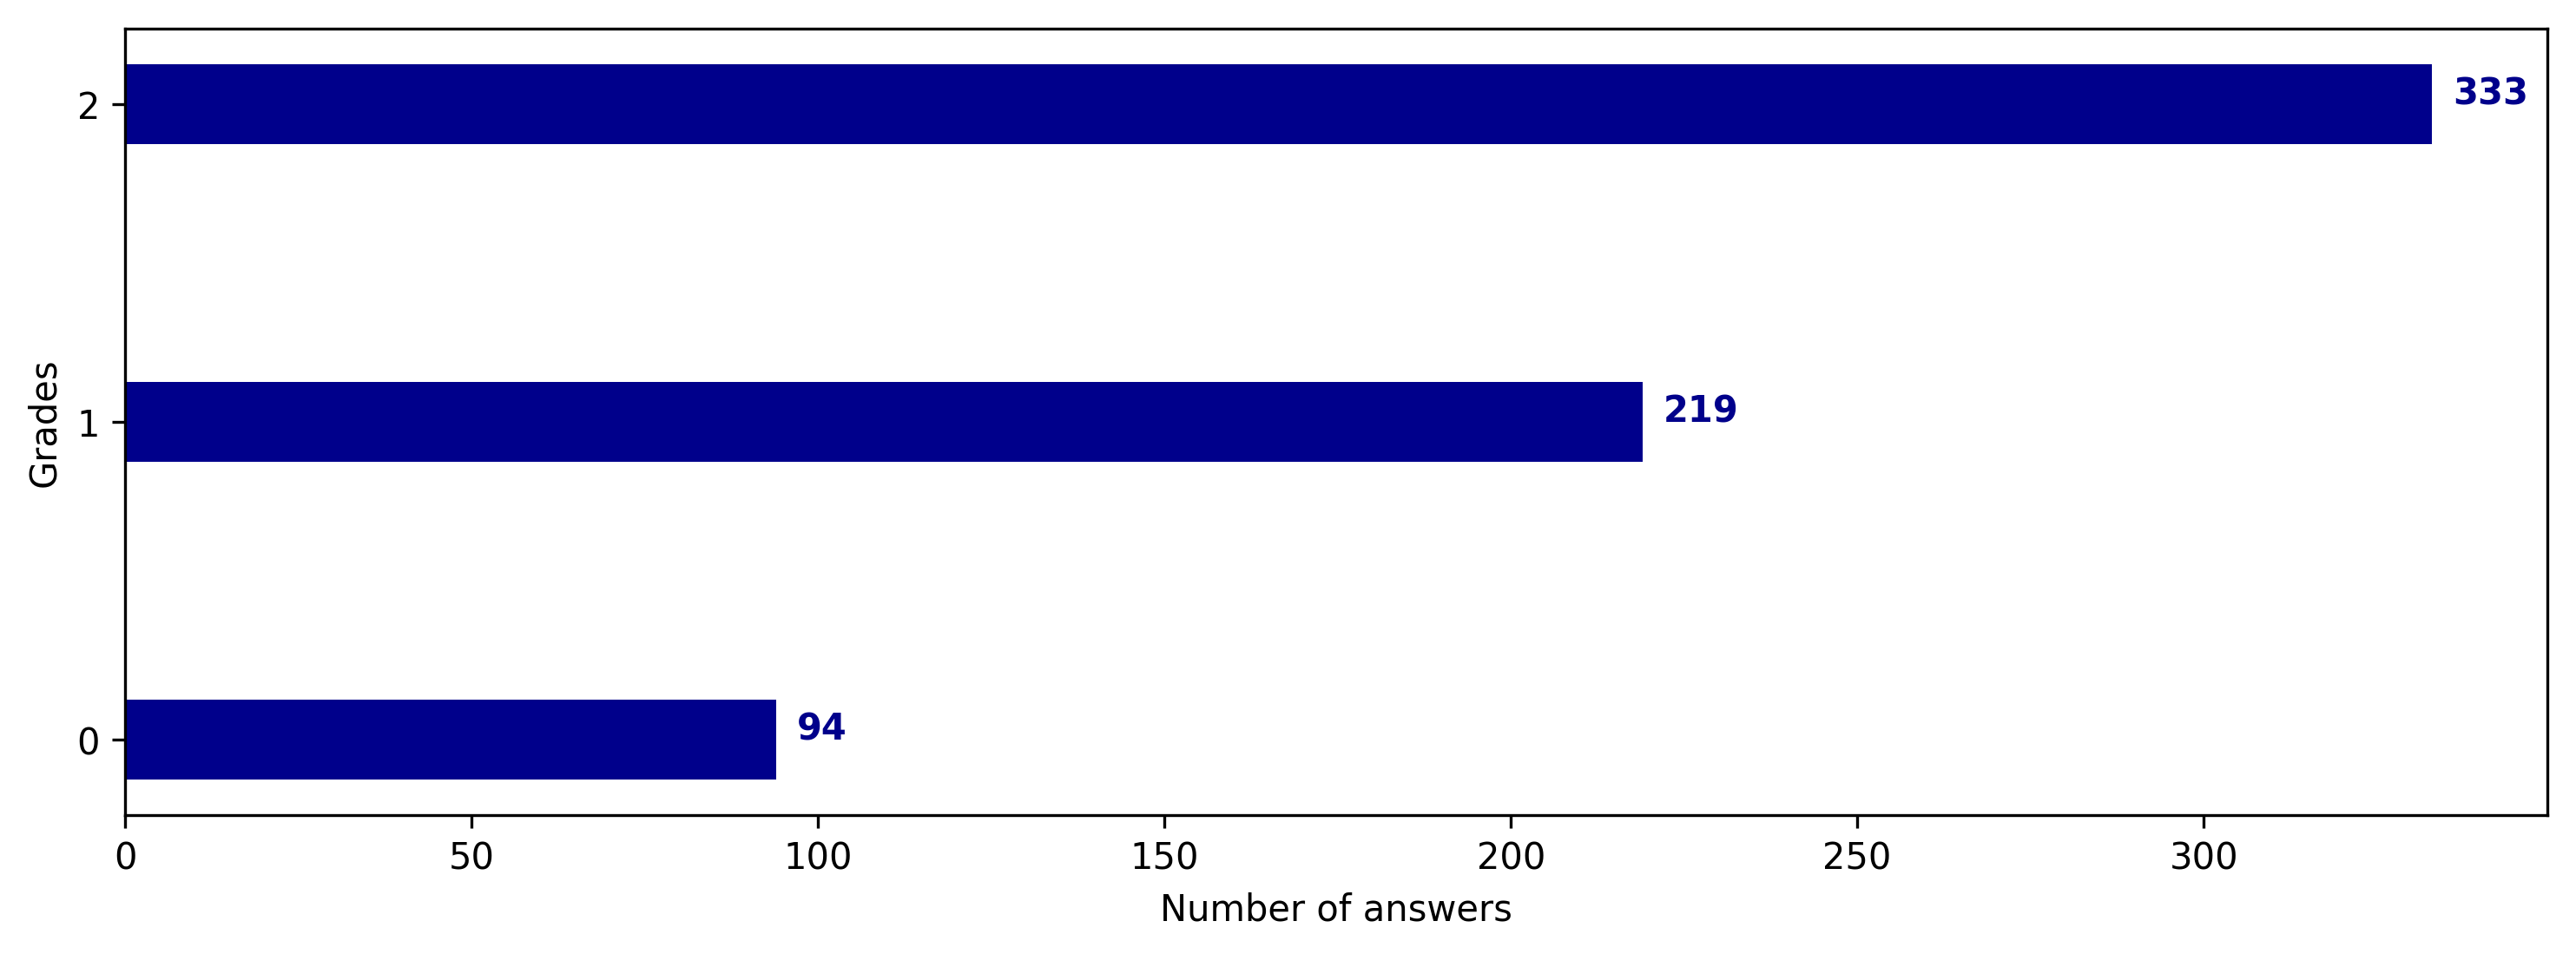
\includegraphics[scale=0.3]{images/nngrades}
		\caption{Grade distribution of the Neural Network dataset}
		\label{nngrades}
	\end{figure} 

	The overall objective of this research is to utilize the autograding models for in-house assignments and examinations. Hence, the answers of students for the Neural Networks course were included as a dataset for this task.
	
	\subsection{SemEval-2013 Task 7}
	
	The SemEval-2013 Task 7 consists of two datasets, namely, Beetle dataset and Science Entailment Corpus (SciEntsBank) dataset. The latter one is used in the experiments of this project. SciEntsBank dataset is a collection of student answers to Science assessment questions compiled by Nielson et al. 2008 \cite{nielsen2008annotating}. This consists of 10804 question answer pairs which are divided into four sections. The first section consists of 4969 answers which are meant to be used as training set. The second section consists of 540 answers which are unseen when compared to the training set. The third section of answers consists of 4562 answers which does not have any common questions with the training set. The fourth section consists of answers which belongs to a totally different domain than the ones in the other three sections. In contrast to the datasets mentioned before, this dataset has five classes, namely, correct, partially correct incomplete, contradictory, irrelevant, and unknown domain \cite{dzikovska2013}. 
	
	In this project, we mapped these classes into numeric grades as;
	
	\{correct:0, partially correct incomplete:1, contradictory:2, irrelevant:3, and unknown domain:4\} 
	
	The class distribution of these four subsections of this dataset are shown in Fig \ref{semevalgrades}.
	
	
	
	\begin{figure}
		\centering
		\begin{subfigure}[b]{0.4\textwidth}
			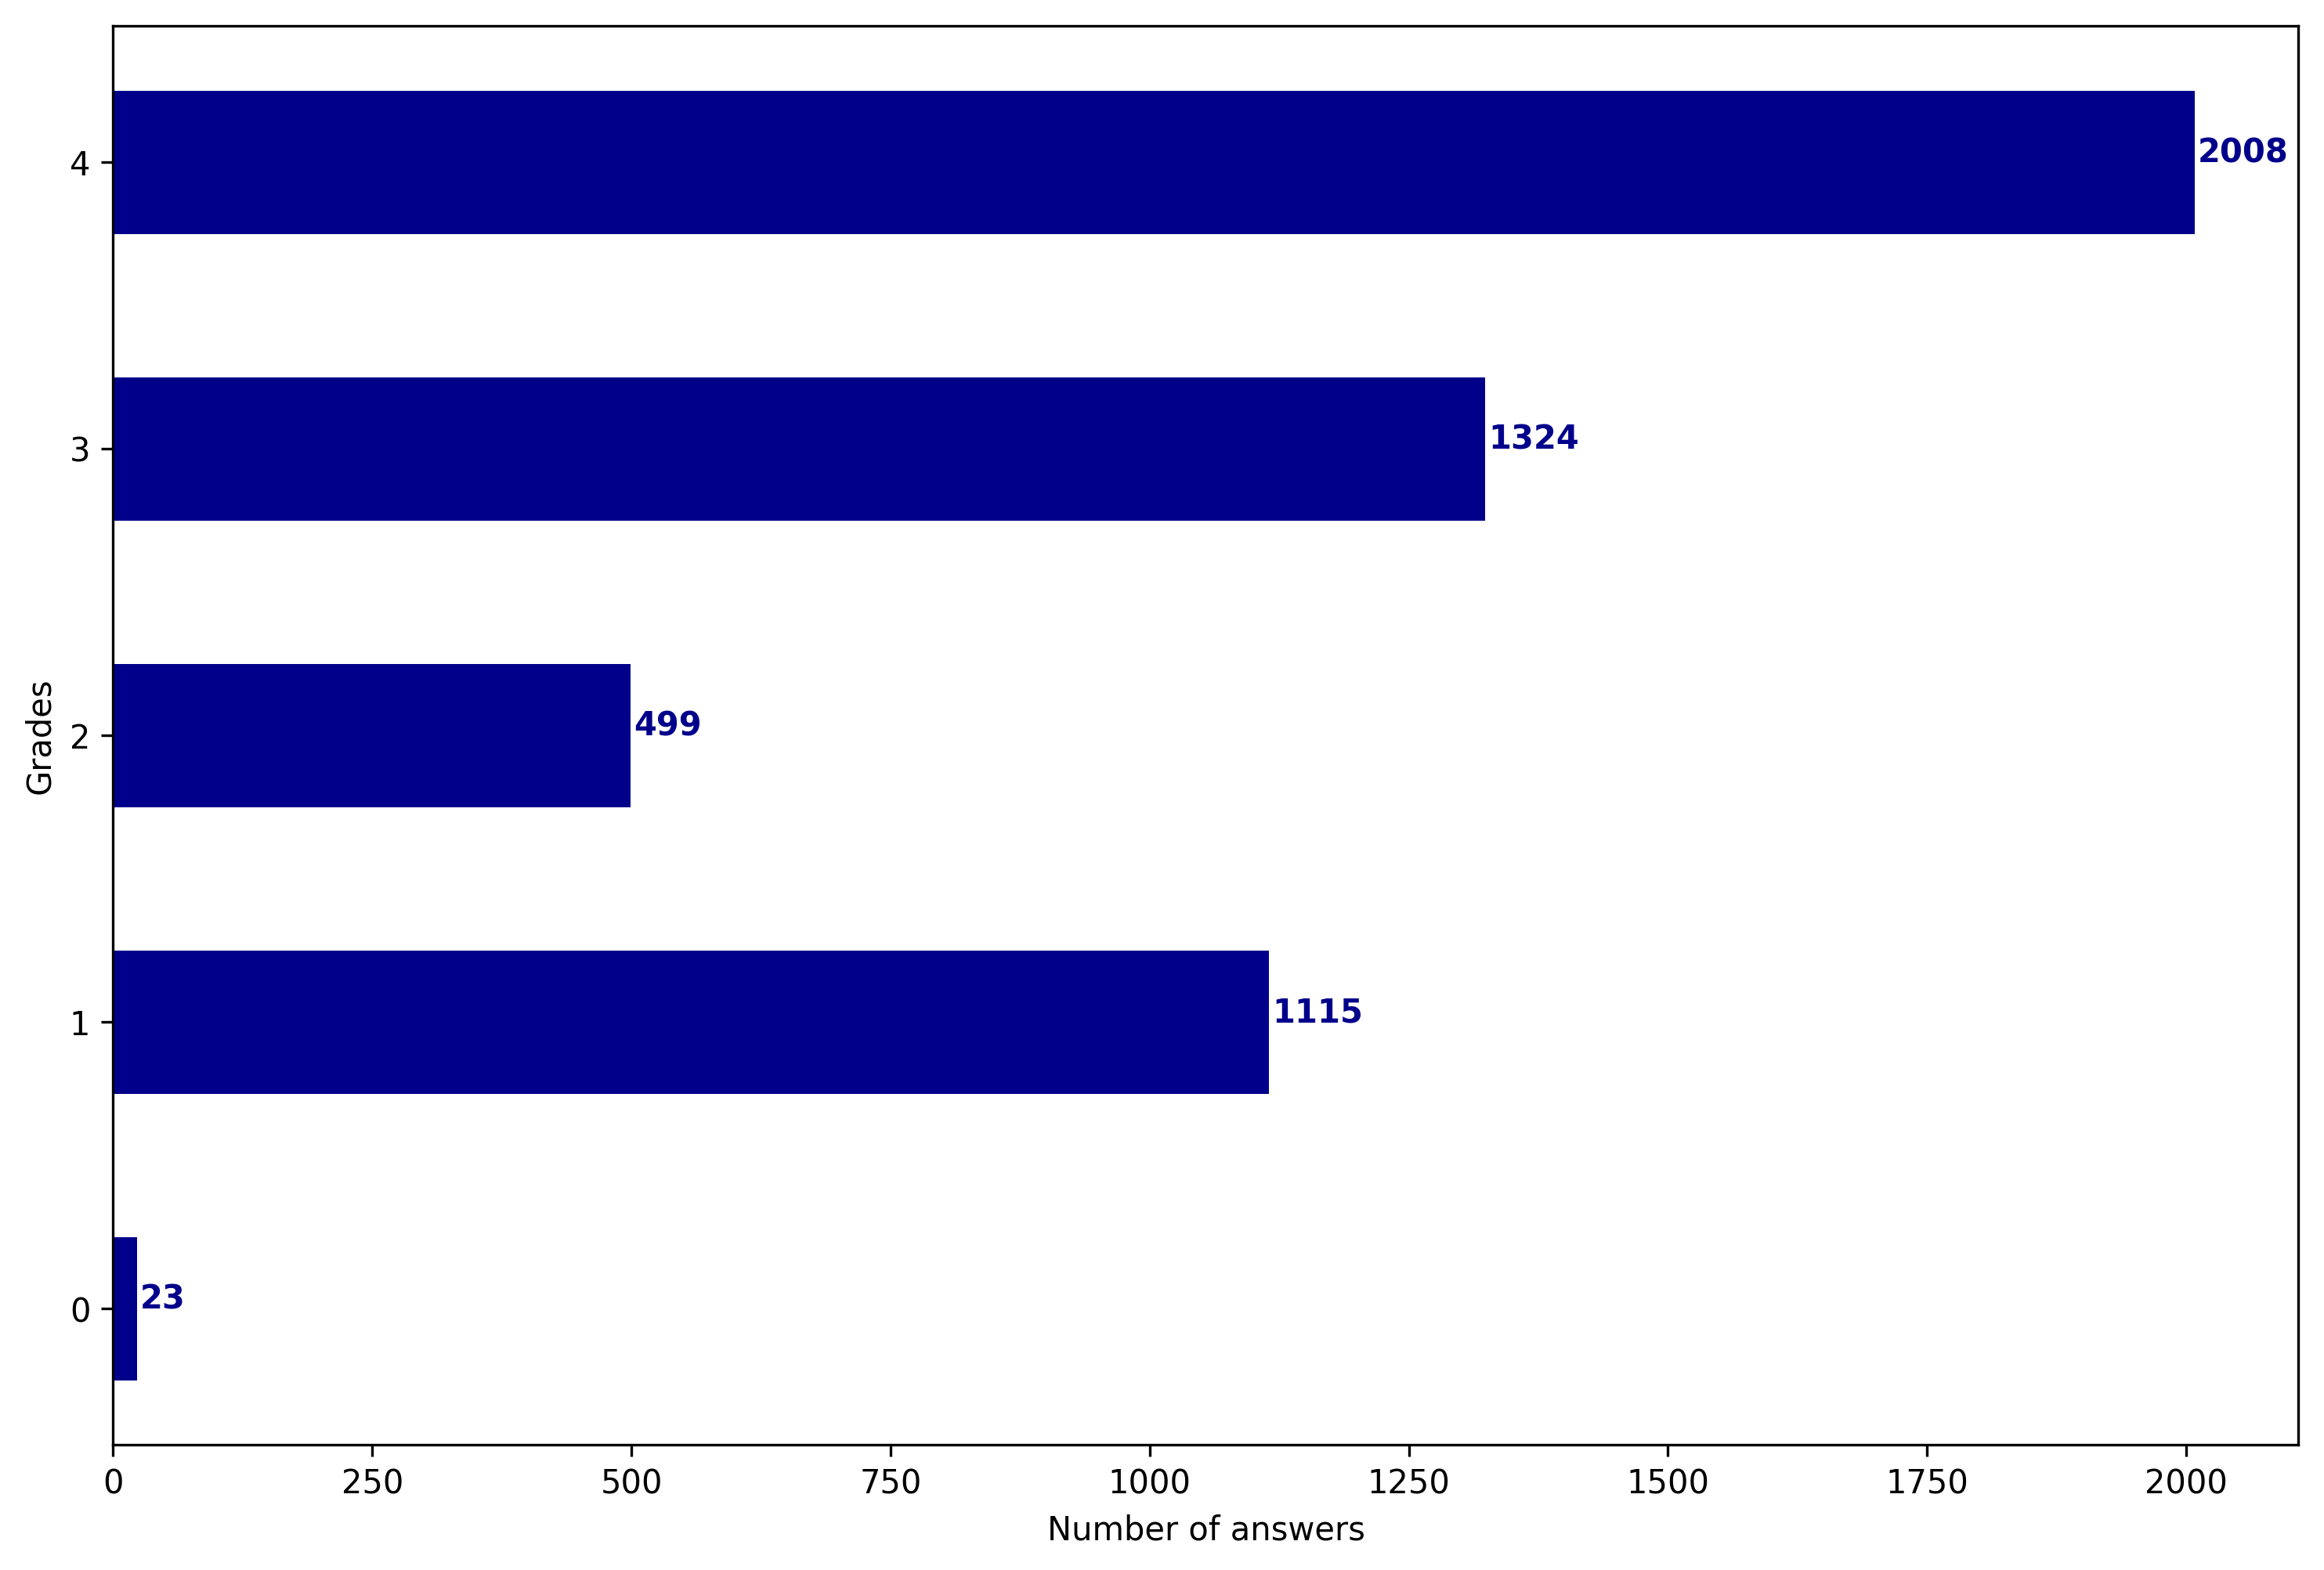
\includegraphics[width=\textwidth]{images/semevalgrades}
			\caption{Train dataset}
		\end{subfigure}
		~
		\begin{subfigure}[b]{0.4\textwidth}
			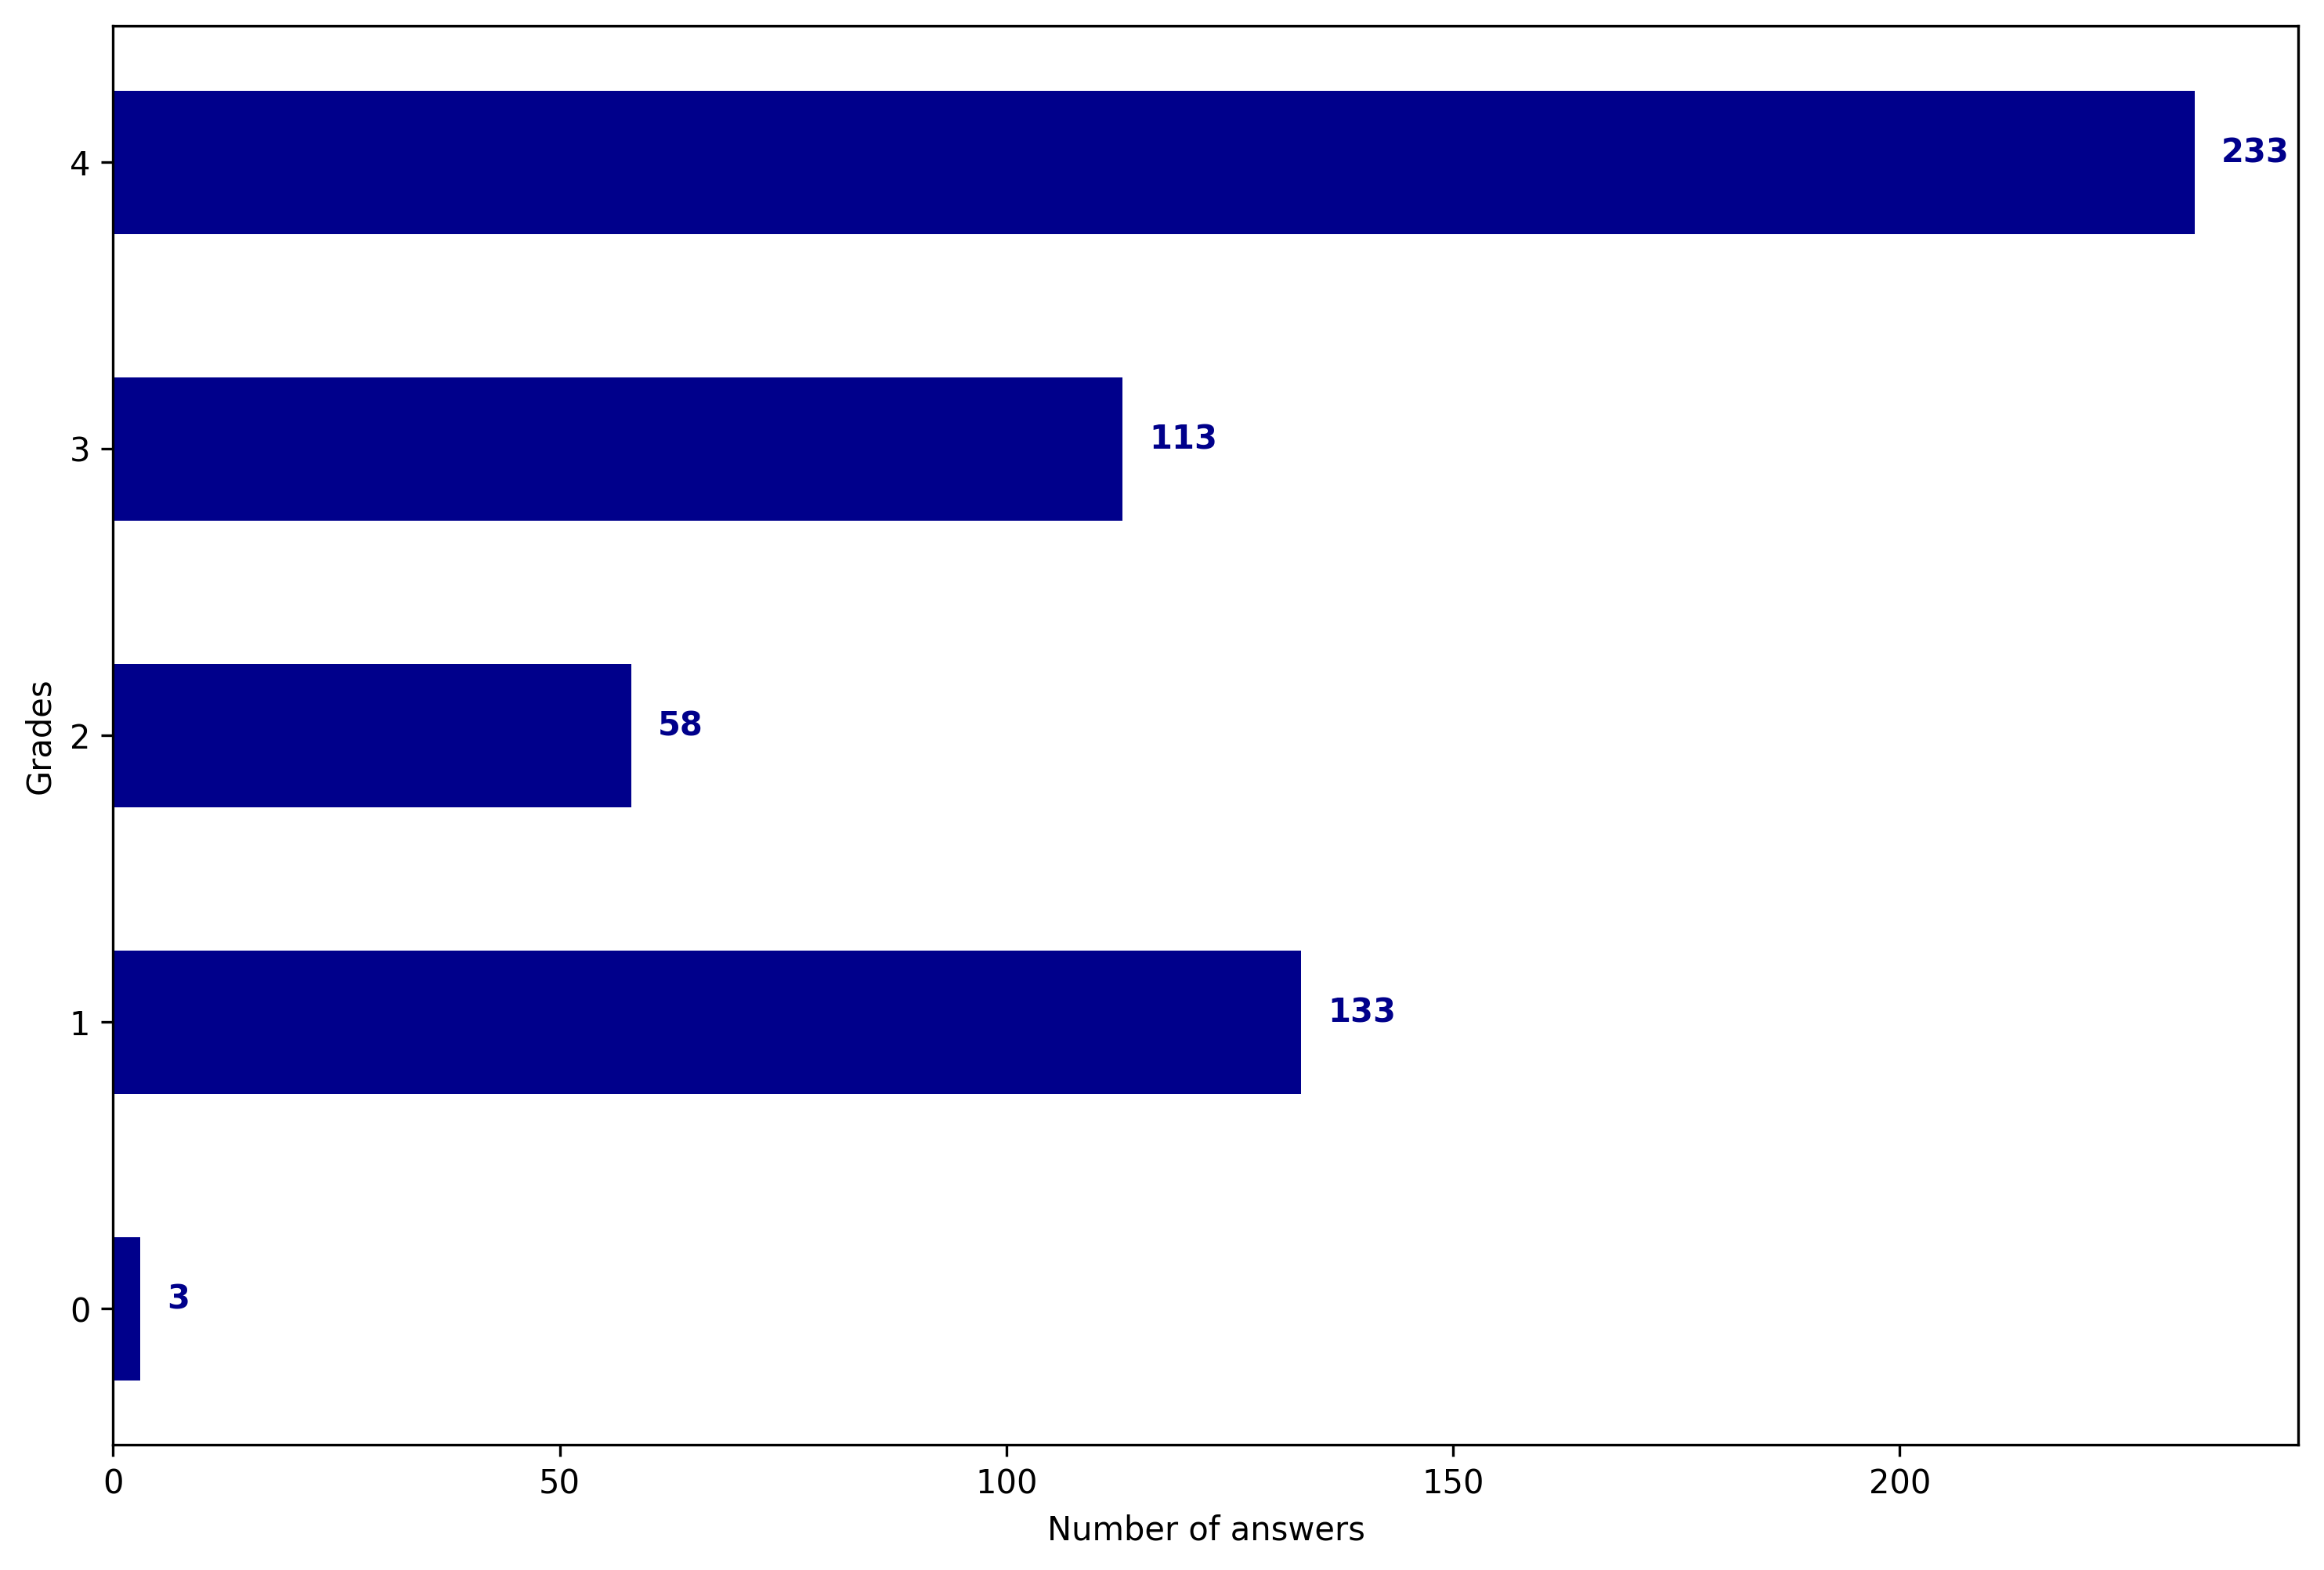
\includegraphics[width=\textwidth]{images/semevalt1grades}
			\caption{Test - unseen answers}
		\end{subfigure}
		
		~
		\begin{subfigure}[b]{0.4\textwidth}
			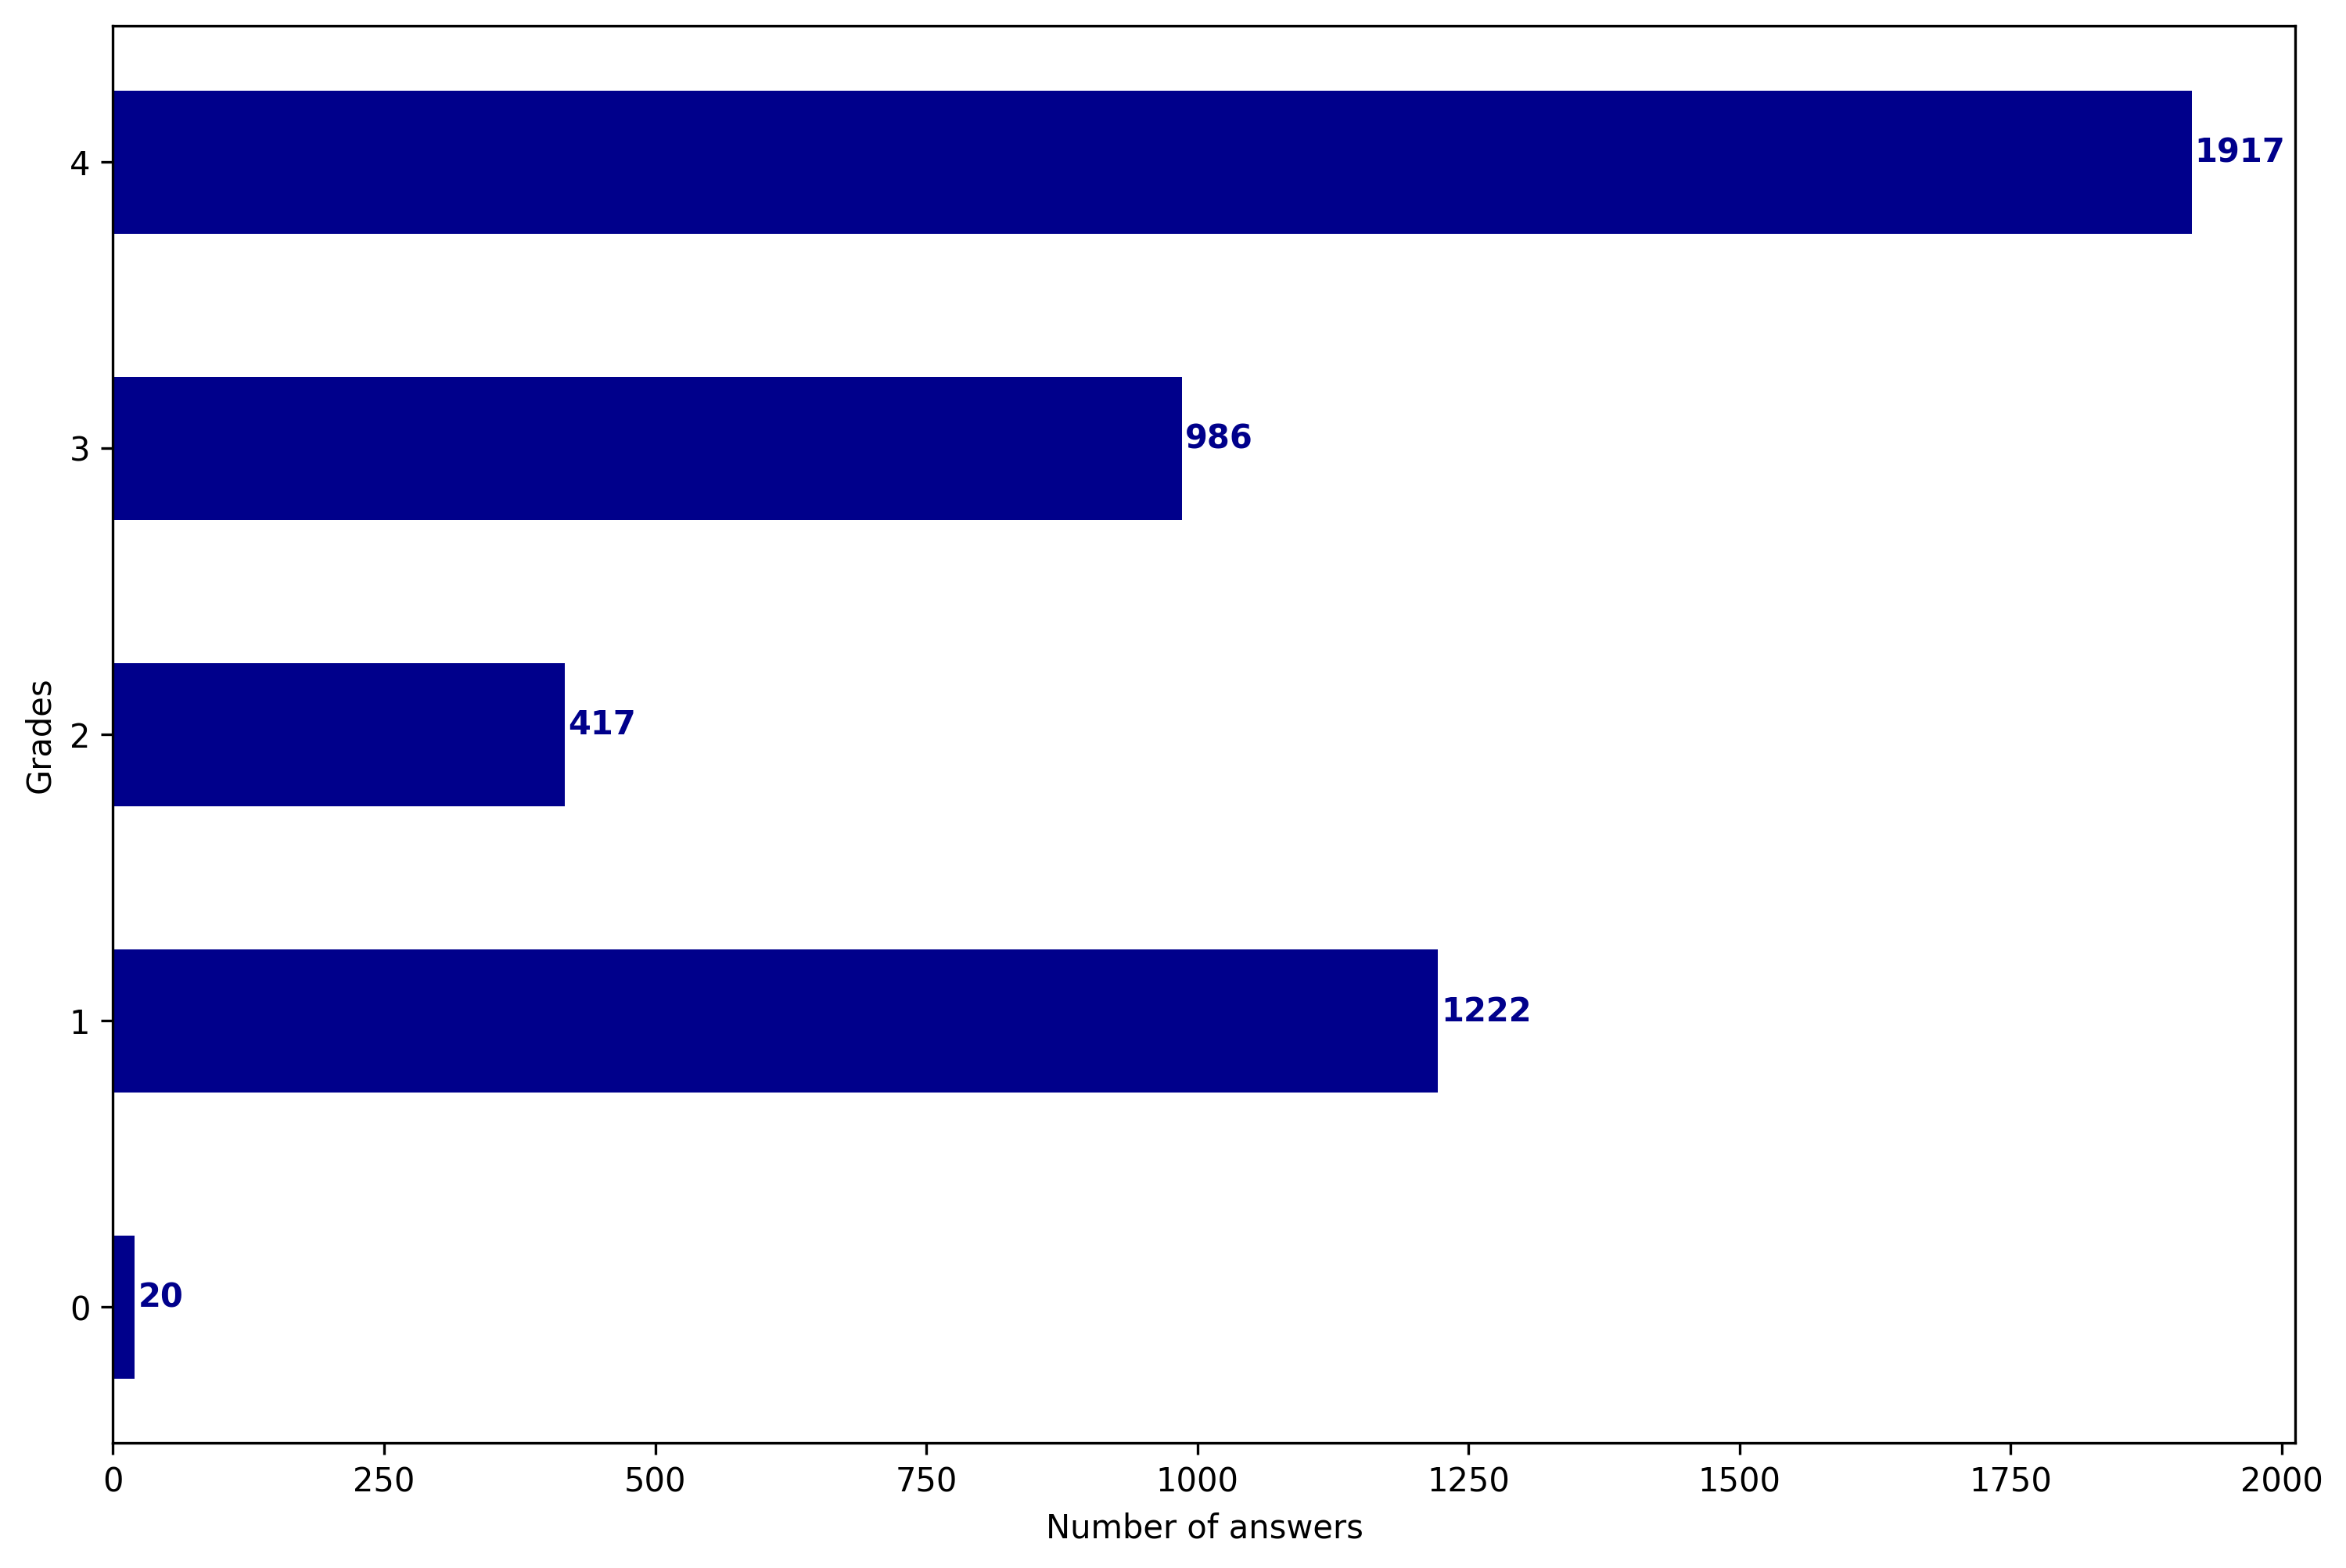
\includegraphics[width=\textwidth]{images/semevalt2grades}
			\caption{Test - unseen domains}
		\end{subfigure}
		~ 
		\begin{subfigure}[b]{0.4\textwidth}
			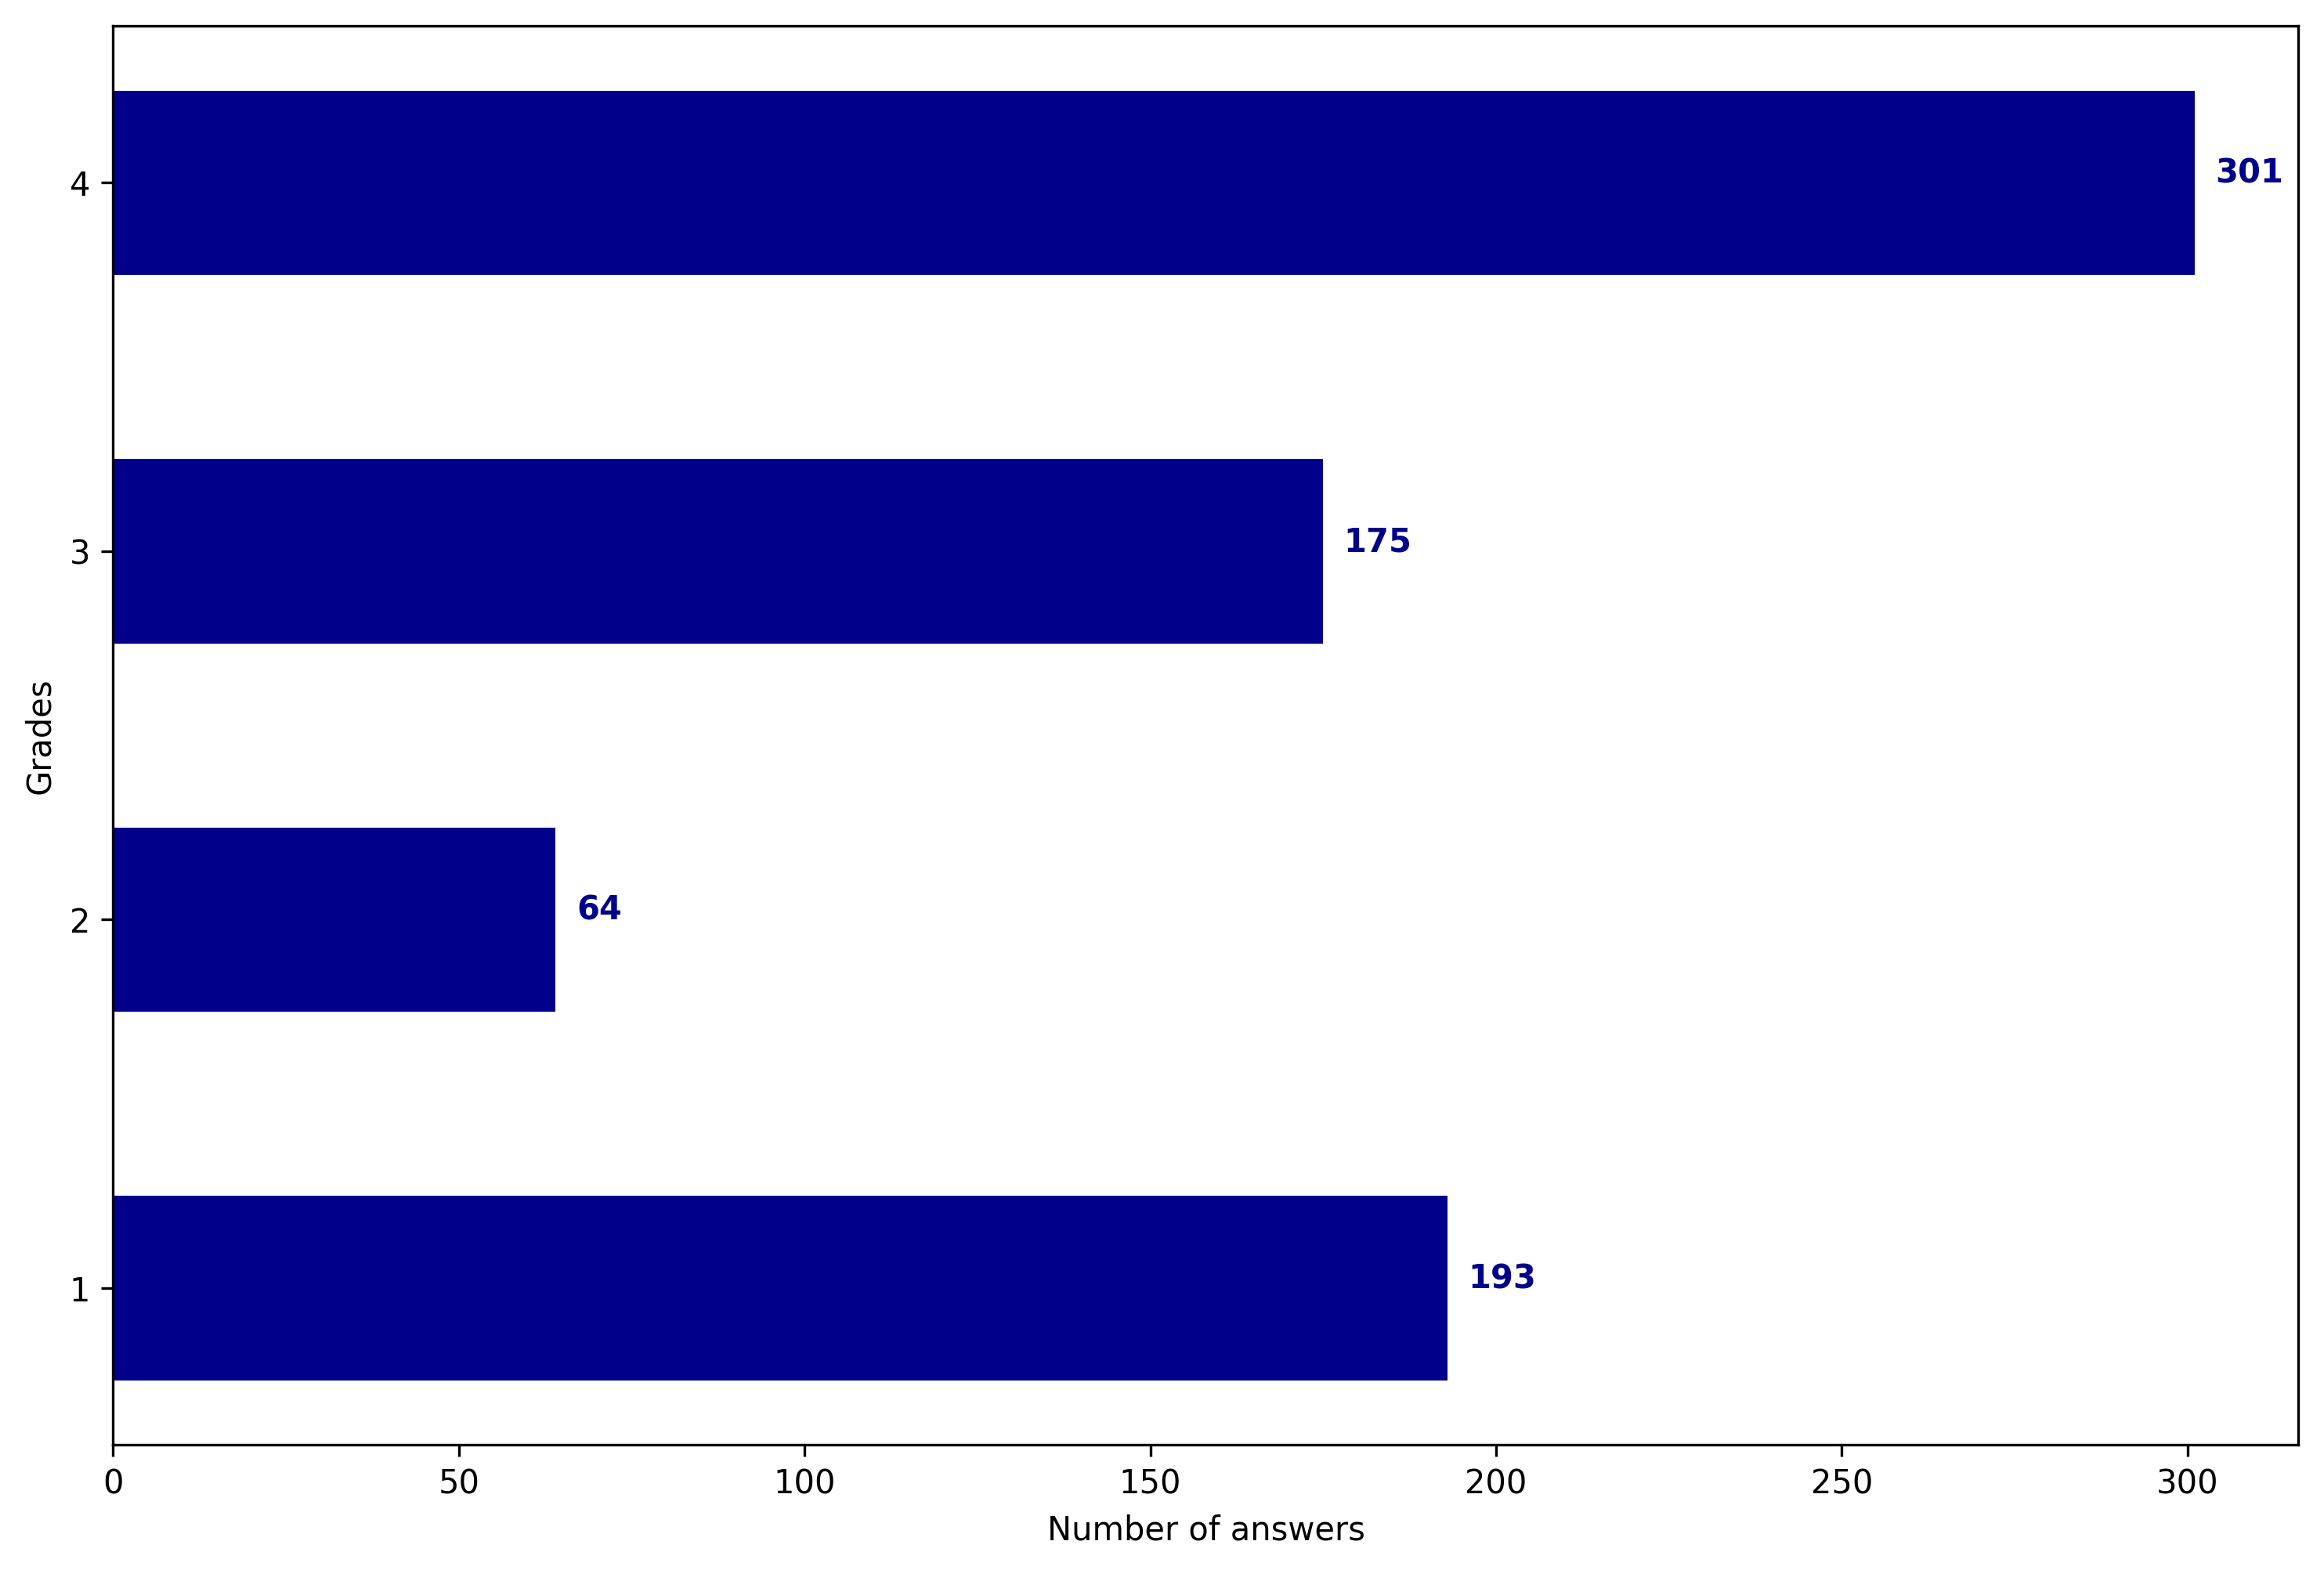
\includegraphics[width=\textwidth]{images/semevalt3grades}
			\caption{Test - unseen questions}
		\end{subfigure}
		~ 
		\caption{Grade distribution of SciEntsBank dataset \cite{dzikovska2013}.}\label{semevalgrades}
	\end{figure}
	
	One of the unique features of this dataset is that it belongs to a different domain than the first two dataset. In addition, the fact that the test dataset has been explicitly divided into unseen answers, unseen questions and unseen domains which facilitates evaluating the generalization ability of the trained model. Recent researches done in ASAG have used this dataset for their evaluations \cite{liu2016validation} \cite{kumar2017earth}. 
    
    \section{Feature Extraction}
    
    Feature extraction deals with getting the relavant features from the raw dataset. The first task involves bringing all the raw data into a common format. In this research work, all the raw data were converted into a comma separated values (csv) file format so that it could be fed into a pandas dataframe. Five main features were extracted from the dataset consisting of questions, student answers, reference answers and their grades in order to feed them into our machine learning models. These features were stored as columns in the dataframe which facilitates using different collection of them while training a machine learning model. Having the data in a pandas dataframe enables faster processing of the data and efficient extraction of features from them when compared to explicit looping through each and every data sample. In addition, the machine learning library used in this project supports objects of type dataframe. Cleaning each of the dataset and the process of converting it into a pandas dataframe format is discussed below. 
    
    \textbf{Mohler'11 Dataset} - This dataset was downloaded from \url{http://web.eecs.umich.edu/~mihalcea/downloads/ShortAnswerGrading_v2.0.zip}, which was available in a text file (.txt) format. The student answers for each question, reference answers and questions were in separate files. A script was written to collect the questions, their corresponding student and reference answers. Later they were converted into a csv file which is stored as a pandas dataframe. Each row of the csv file consists of the question id, question, student's answer, reference answer and the grade. The first 5 lines of this dataframe is shown in Fig \ref{mohler_df}.
    
    \begin{figure}[h]
    	\centering
    	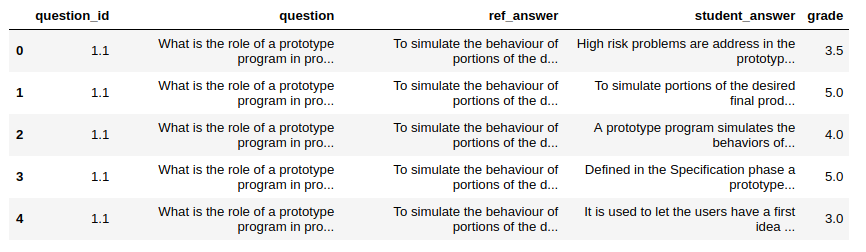
\includegraphics[scale=0.4]{images/mohler_df}
    	\caption{Dataframe of Mohler'11 dataset.}
    	\label{mohler_df}
    \end{figure} 
    
    The features were extracted from this dataframe.
    
    \textbf{Neural Network dataset} - The student answers from the final semester exam of Neural Networks course in Hochschule Bonn-Rhein-Sieg were collected by the Professor and the teaching assistant of the course. Each student wrote his/her answers in a \href{jupyter.org}{Jupyter Notebook} file as shown in Fig \ref{nn_notebook}. 
    
    \begin{figure}[h]
    	\centering
    	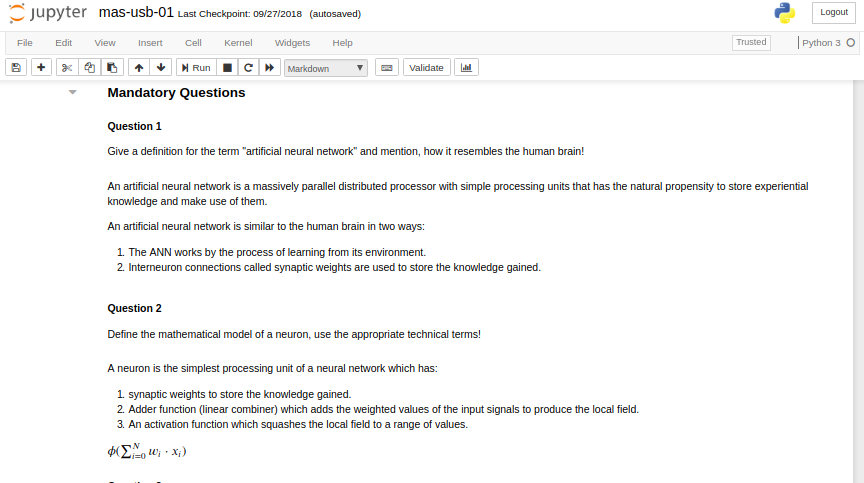
\includegraphics[scale=0.4]{images/nn_notebook}
    	\caption{Example of a student submission in jupyter notebook.}
    	\label{nn_notebook}
    \end{figure} 
    
    The grades were entered in a separate spreadsheet file. The reference answers were constructed from the keywords provided by the Professor for the manual grading purpose. A script was written to parse these notebook files, spreadsheet of keyword answers, and the spreadsheet of grades into a csv file format similar to the Mohler'11 dataset. The first 5 lines of the dataframe constructed from this csv file is shown in Fig \ref{nn_df}. The features were extracted from this dataframe.
    
    \begin{figure}[h]
    	\centering
    	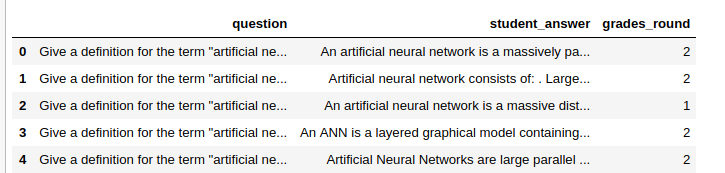
\includegraphics[scale=0.4]{images/nn_df}
    	\caption{Dataframe of Neural Network dataset.}
    	\label{nn_df}
    \end{figure} 
    
    \textbf{SemEval-2013 Task 7} - This dataset was from a \href{https://www.cs.york.ac.uk/semeval-2013/task7/}{textual entailment challenge} which has questions and student answers in different domains. These files were found in a eXtensible markup language (xml) file format. Each file contains a questions, its reference answer, the students' answers and their corresponding grades as shown in Fig \ref{semeval_xml}. 
    
    \begin{figure}[h]
    	\centering
    	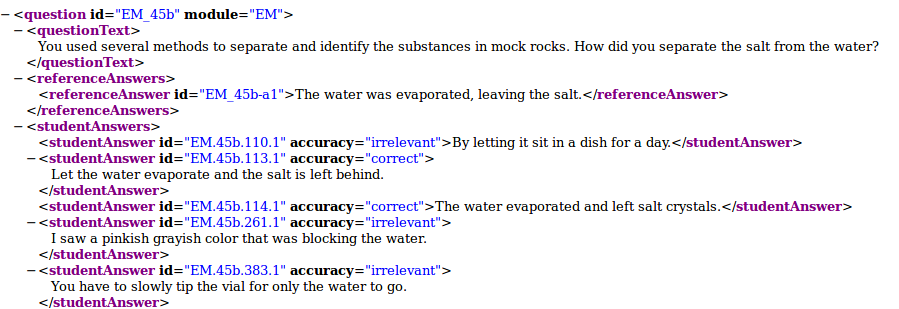
\includegraphics[scale=0.4]{images/semeval_xml}
    	\caption{SemEval-2013 Task 7 dataset in xml format.}
    	\label{semeval_xml}
    \end{figure}
    
    These xml files were converted into a csv file with the help of a script file. The first 5 lines of the dataframe constructed from this csv file similar to the Mohler'11 dataset as shown in Fig \ref{semeval_df}. The features were extracted from this dataframe.
    
    \begin{figure}[h]
    	\centering
    	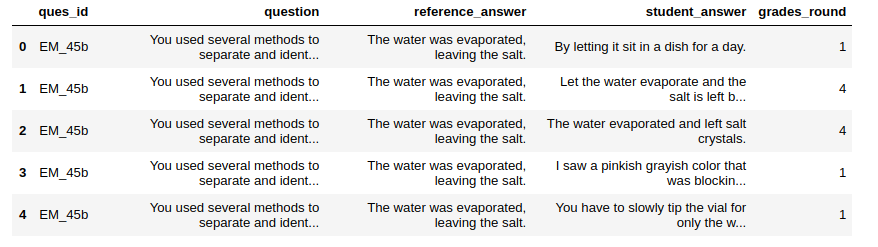
\includegraphics[scale=0.4]{images/semeval_df}
    	\caption{Dataframe of SemEval-2013 Task 7 dataset.}
    	\label{semeval_df}
    \end{figure} 
    
    \subsection{Bag-of-Words(BOW)}
    
    The following preprocessing tasks were done before converting all the student answers into bag-of-words.
    
    \begin{itemize}
    	\item Converting into lowercase
    	\item Removing the punctuations
    	\item Stop words removal
    	\item Lemmatization 
    \end{itemize} 
    
    After performing all these tasks, the answers were brought into a common format. The bag-of-words representation of the answers were obtained using sklearn library's \href{https://scikit-learn.org/stable/modules/generated/sklearn.feature_extraction.text.CountVectorizer.html}{CountVectorizer}. This technique returns a sparse matrix of count numbers after considering all the answers and building a vocabulary of tokens in them. This process is done efficiently when feeding the answers in a \href{https://pandas.pydata.org/pandas-docs/version/0.23.4/generated/pandas.Series.html}{pandas Series} format.
    
    For e.g., tokens extracted from the first sentences of three answers from the Neural Network dataset 'artificial neural network massively parallel distributed processor', 'artificial neural network largely parallel distributed processor', and 'artificial neural network consists neurons' would be;
    
    
    ['artificial', 'consists', 'distributed', 'largely', 'massively', 'network', 'neural', 'neurons', 'parallel', 'processor']
    
    
    The bag-of-words matrix constructed from these answers based on the tokens shown above would be as follows;
    
     {\footnotesize  $$ \begin{bmatrix}
     	1 & 0 & 1 & 0 & 1 & 1 & 1 & 0 & 1 & 1 \\
     	1 & 0 & 1 & 1 & 0 & 1 & 1 & 0 & 1 & 1 \\
     	1 & 1 & 0 & 0 & 0 & 1 & 1 & 1 & 0 & 0
     	\end{bmatrix}  $$}   

    \subsection{Term Frequency-Inverse Document Frequency (tf-idf)}
    
    Similar to the bag-of-words model, tf-idf constructs sparse matrix for student answers based on the word frequencies of the unique tokens. Tf-idf takes the most important words into account and weights unimportant words less. Hence, the presence of keywords and subject specific terms have more chance of being explicitely represented in the tf-idf matrix. The preprocessing steps before converting the answers into tf-idf format is similar to that of bag-of-words. Here the sklearn library's \href{https://scikit-learn.org/stable/modules/generated/sklearn.feature_extraction.text.TfidfVectorizer.html}{TfidfVectorizer} tool is used for the construction of the matrix. The tf-idf matrix for the same three answers of the Neural network dataset is shown below.
    \vspace{3mm}
    
   {\tiny  $$ \begin{bmatrix}
    
   0.30371 & 0.  & 0.39108 & 0 &  0.51423  & 0.30371 & 0.30371 & 0 & 0.39108 & 0.39108 \\
   
   0.30371 & 0. & 0.39108 & 0.51423 & 0. &  0.30371 &  0.30371 & 0. & 0.39108 & 0.39108 \\
   
   0.33838  & 0.57292 & 0. & 0. & 0. & 0.33838 & 0.33838 & 0.57292 & 0. & 0.
   
    \end{bmatrix}  $$} 
	
	\subsection{Features from Sultan et al., 2016 \cite{Sultan2016}}
	
	The state-of-the-art supervised learning model for short answer grading system used five different features for learning and those features are experimented in this work too. The features are mainly based on text similarity between the students' answers and the corresponding reference answers. These features in the supervised learning model were used for a regression task whereas the features are used in an active learning setup for a classification task in this project. The five main features are as follows, and these will be explained in detail below. 
	
	\begin{itemize}
		\item Length Ratio
		\item Word Alignment
		\item Semantic Vector Similarity
		\item Word Alignment (with question demoting)
		\item Semanctic Vector Similarity (with question demoting)
	\end{itemize}  
	
	Question demoting is the task of removing words that appear in the question from the reference answer and the student answer. This is done in order to reduce the possibility of earning more grades just by repeating the words in the question \cite{Sultan2016}. Fig \ref{sultan_features} illustrates how the student answers and reference answers are converted into a feature array of five columns which is then fed into a machine learning model. Every feature column is normalized using scikit-learn's \href{https://scikit-learn.org/stable/modules/generated/sklearn.preprocessing.MinMaxScaler.html}{MinMaxScaler} before using them in the model to avoid bias towards a particular feature.
	
	\begin{figure}[h]
		\centering
		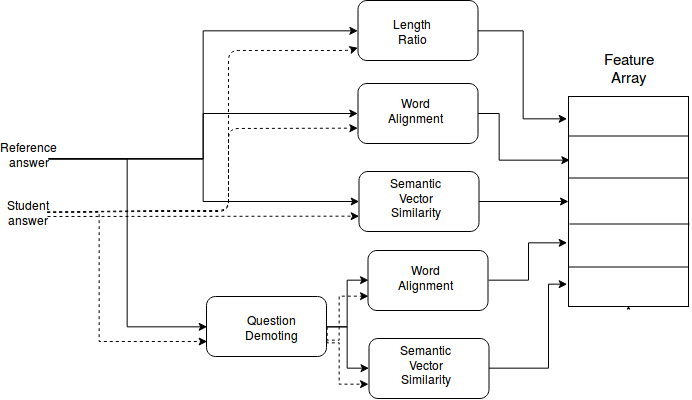
\includegraphics[scale=0.4]{images/feature_array}
		\caption{Block diagram of construction of feature array. Image adapted from \cite{ramesh2} \cite{Sultan2016}.}
		\label{sultan_features}
	\end{figure} 
	
	\subsubsection{Length Ratio}
	
	This feature tries to combat the chances of providing high grades for students answers which are intentionally written in a long format without proper content in it. The feature value was calculated by dividing the student answer's length by the reference answer's length. For e.g., a student's answer from the Mohler'11 dataset \cite{Mohler2011}, the corresponding reference answer, and the length ratio is as follows; \\
	
	\noindent \textbf{Reference answer}: 'To simulate the behaviour of portions of the desired software product.' \\
	\textbf{Student answer}: 'To simulate portions of the desired final product with a quick and easy program that does a small specific job.  It is a way to help see what the problem is and how you may solve it in the final project.'\\
	\textbf{Length Ratio}: 0.268 (11/41)
	
	
	\subsubsection{Word Alignment \cite{sultan2014back}}
	
	In order to capture the semantic similarity between the student answer and the reference answer, each pair of words from both the sentences are considered for scoring based on their contextual and lexical similarity the the scores of all those pairs were combined in the form of a weighted sum to calculate a final alignment measure. Paraphrase database \cite{ganitkevitch2013ppdb} was used to measure how a pair of words are similar lexically. Dependency measures are employed to capture the contextual similarity of a pair of words. For e.g., a word in a student's answer and another word in the reference answer is processed for their dependencies in the respective sentences and the calculated score was weighted in the final calculation of the final alignment score. 
	
	The original implementation of word alignment by \cite{sultan2014back} utilized Stanford CoreNLP. A fellow research student in our \href{https://digiklausur.github.io/}{E-assesment team}, Ramesh Kumar implementated the same algorithm using NLTK and achieved similar results \cite{ramesh2}. We have used Ramesh's NLTK implementation for getting the word alignment score in our datasets. For e.g., a reference answer, a student's answer in the Semeval dataset \cite{nielsen2008annotating} and the aligned words are as shown below; \\ 
	
	
	\noindent \textbf{Reference answer}: 'The water was evaporated, leaving the salt.' \\
	\textbf{Student answer}: 'Let the water evaporate and the salt is left behind.' \\
	\textbf{Aligned words}: [['evaporated', 'evaporate'], ['water', 'water'], ['salt', 'salt'], ['leaving', 'left']]    
	
	Similar alignment scores were calculated for every pair of question demoted student and reference answers and added as a separate feature in the feature array.	
	
	\subsubsection{Semantic Vector Similarity}
	Cosine similarity is one of the mathematical techniques to find the similarity between two vectors. Two vectors which point in the same direction and have a small angle between them would have a high cosine similarity than two vectors which point in opposite directions. This measure could be utilized for texts as well. When the cosine similarity of two sentences (which are converted into vectors by some means) is high, it could be inferred that there is a high chance of them having the same meaning \cite{cos_sim}. Semantic vector similarity is a score calculated based on the cosine similarity between the vectors of the student and reference answers.       
	
	In order to compute the cosine similarity, the student and the reference answers were converted into word vectors using the \href{https://radimrehurek.com/gensim/models/word2vec.html}{gensim word2vec} model. Each word in a student and reference answers was converted into a 400 dimensional vector and they were summed up for each sentence. The cosine similarity was calculated between these vectors using \href{https://docs.scipy.org/doc/scipy/reference/generated/scipy.spatial.distance.cosine.html}{scipy.spatial} library in order to produce a score for the semantic vector similarity feature. Similar kind of vectors were calculated for question demoted versions of student and reference answers the cosine similarity between these two vectors was used as another feature in the feature array.
    
    \section{Machine Learning Models \cite{raschka2015python}} 
    
    The machine learning models used in this project are implemented with the help of the scikit-learn library \cite{scikit_learn}.
    
    \subsection{Logistic Regression}
    
    Logistic regression is widely used for classification problems which is most suitable for classifying linearly separable data. In a simple binary classification task, the model calculates the weight for each sample such that;
    
    \begin{equation}  
    P(y=1|x) = \sum_{i=0}^{m} w_i x_i
    \end{equation} 
    
    where the $w_i$ is the weight for the $i^{th}$ feature and $x$ is the sample. The weights are learned from the training samples by minimizing the cost function (a measure of how the predictions are off from the actual outcome) using the gradient descent method. Taking $\sum_{i=0}^{m} w_i x_i$ as $z$, the model calculates the probability that a given sample belongs to a particular class using the sigmoid function(logistic function) as shown below.  
    
    \begin{equation}  
    \phi(z) = \frac{1}{1+e^{-z}} 
    \end{equation} 
    
    The resulting value is compared against a threshold to decide whether the sample belongs to the positive or negative class. Similarly, the model works in multi-class settings by considering one class as positive and all other classes as negative (one vs. rest strategy). 
    
     
    \subsection{Naive Bayes Classifier}
    
    Naive Bayes classifier calculates the probability of each sample belonging to a particular class by taking into account every feature of the sample independently (the independence assumption of each feature causes the name "naive"). From the training samples, it calculates the probability of each feature given the class ($P(x_i|C_i)$) and the class distribution of all the samples. With this information, it calculates the class for a new sample by using the Bayes' theorem as stated below.
    
    \begin{equation}
    P(C_i | x) = \frac{P(x|C_i) P(C_i)}{P(x)}
    \end{equation}  
    
    For applications where every feature could take multiple values, a multinomial Naive Bayes (generalization of binary Naive Bayes) is used. This model is known for its simple implementation and good performance with less data. 
    
    \subsection{Random Forests}
    
    Random forests is a bag of decision trees (ensemble learning of decision trees) which makes a prediction after considering the vote of each decision tree in the ensemble. Each decision tree builds a tree with features as branching factors and splits the samples based on the decisions made by the branching factor. Every branching factor (a feature of the sample) splits the samples according to the value of that particular sample using a threshold (for ex., left if the value is lesser than the threshold or right if it's more than the threshold). The features to be considered at every branching point is decided based on how informative or useful it is to split the samples based on that feature. Information gain is one of the metrics used to find the most informative features. The features and the decision thresholds are learned from the training samples and it is applied to the test samples.
    
    Though random forests are difficult to interpret, they are known for dealing with multiple features which could be correlated, and reduced variance. 
    
    
    \subsection{Support Vector Machines}    
    
    Support Vector Machines (SVM) are models which define a decision boundary such that the data are linearly separated. Fig \ref{svm_graph} shows how an SVM would classify the data with binary classes. The data points which lie along the decision boundary (also known as support vectors) contribute a lot in calculating the parameters of the decision boundary. The model tries to fit the boundary such that the margin between the line and the support vectors are as large as possible so that the model generalizes well (predicts well for unseen data). The model becomes a hyperplane in higher dimensions. 
    
    \begin{figure}[h]
    	\centering
    	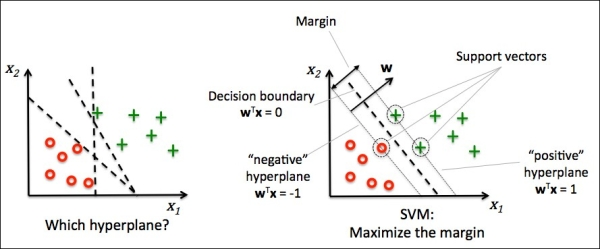
\includegraphics[scale=1.2]{images/svm_graph}
    	\caption{SVM - Hyperplane separating the two classes. Image from \cite{raschka2015python}}
    	\label{svm_graph}
    \end{figure}
    
    In case of nonlinearly separable data, SVM tries to project the data on to a higher dimension and try to fit a hyperplane there such that the data belonging to different classes are separated. Radial Basis Function is one of the kernel methods which is used to project the data onto a higher dimensional feature space. 
    
    \vspace{3mm}
    \section{Experimental Setup}
    
    Experiments were carried out in various settings in order to evaluate the performance of different features, and machine learning models, which could be used within an active learning pipeline. In addition to determining the best features to extract from the answers and the best model to learn the prediction task, the main objective of these experiments is to evaluate the active learning strategies, seed selection mechanism, and batch size during querying for the task of short answer grading.
    
    \subsection{Experiment Pipeline}
    
    Fig \ref{exp_pipeline} illustrates the experimental setup and the different aspects being evaluated in this work.
    
    \begin{figure}[h]
    	\centering
    	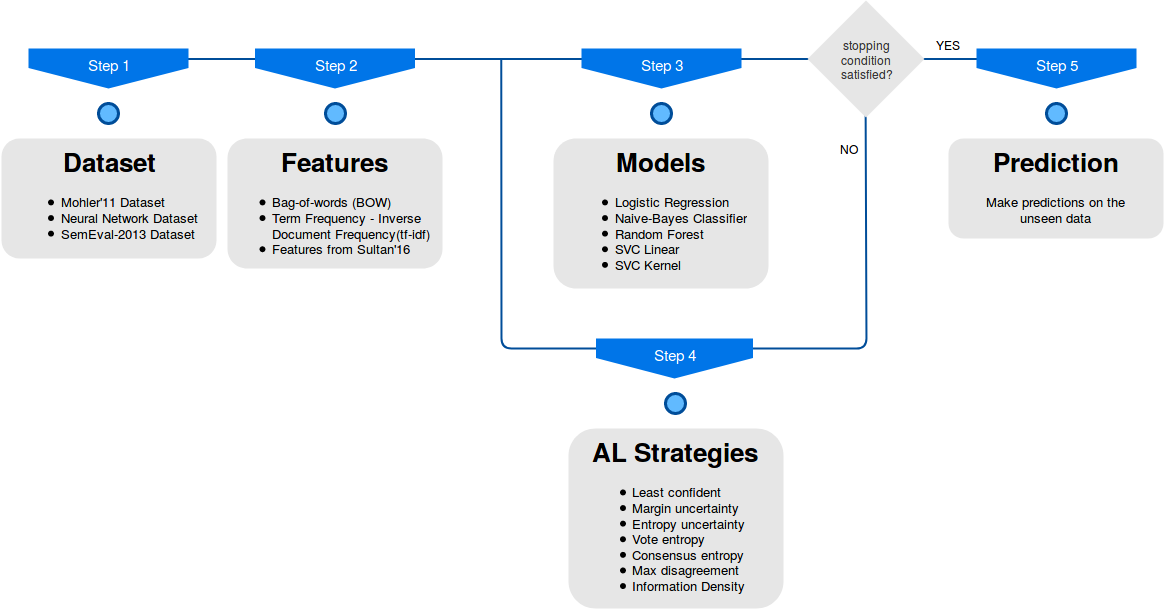
\includegraphics[scale=0.3]{images/experiment_pipeline}
    	\caption{Experiment pipeline of this work.}
    	\label{exp_pipeline}
    \end{figure}
    
    As shown in the figure, every evaluation metric is calculated for a unique setting of features, models, and active learning strategies for every dataset. A large number of experiments were carried out where in every experiment, for every dataset, a feature was fixed and the performance was observed for all different models using different active learning strategies. These experiments were done for both binary and multi-class classifications.  
    
    \subsection{Binary Classification}
    
    Experiments were done considering the task of grading student answers as a binary problem. Each answer was labeled as a correct answer or an incorrect answer based on the actual grade it was awarded. Table \ref{binary_grades} shows how this task of converting the grades into a binary representation was accomplished. 
    
    \begin{table}[h]
    	\centering
    	\begin{tabular}{|c|c|c|}
    		\hline
    		\textbf{Dataset}     & \textbf{Class 1 (correct)} & \textbf{Class 0 (incorrect)} \\ \hline
    		Mohler'11 dataset    & greater than 3.5           & less than or equal to 3.5    \\ \hline
    		SemEval 2013 dataset & greater than 3.0           & less than or equal to 3.0    \\ \hline
    	\end{tabular}
    	\caption{Coversion of grades into binary labels as correct and incorrect.}
    	\label{binary_grades}
    \end{table}
    
    
    Though the grades for both the datasets were on a scale from 0 to 5, the threshold for Mohler'11 dataset was set higher than that of SemEval 2013 dataset as there was a huge inbalance between the high and low grades in it. Increasing the threshold helped in avoiding a large imbalance of the two classes. 
    
    \begin{figure}
    	\centering
    	\begin{subfigure}[b]{0.4\textwidth}
    		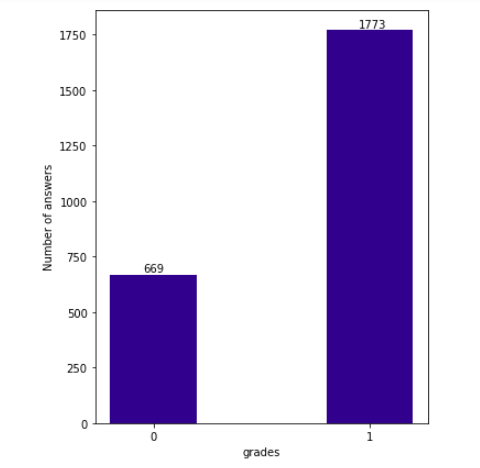
\includegraphics[scale=0.3]{images/mohler_binary_dist}
    		\caption{Binary class distribution of Mohler dataset.}
    		\label{mm_binary_dist}
    	\end{subfigure}
	    ~
	    \begin{subfigure}[b]{0.4\textwidth}
	    	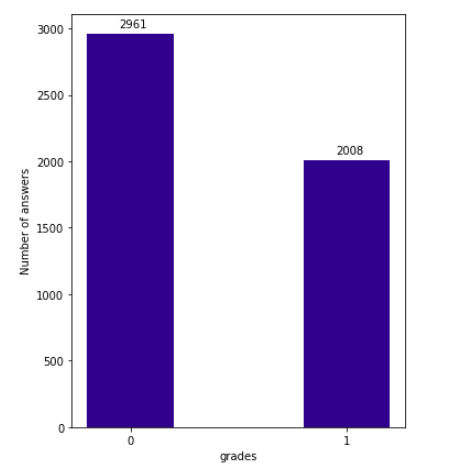
\includegraphics[scale=0.3]{images/semeval_binary_dist}
	    	\caption{Binary class distribution of SemEval 2013 dataset.}
	    	\label{semeval_binary_dist}
	    \end{subfigure}
	    \caption{Binary class distributions.}
    \end{figure}
    
    Fig \ref{mm_binary_dist} and Fig \ref{semeval_binary_dist} show the class distributions after the conversion. Binary classification task was not performed on the Neural Network dataset as it had only 3 classes and it was difficult to split them into correct and incorrect answers. 
    
    \subsection{Multi-class Classification}
    
    As opposed to Binary classification, the real world application includes awarding grades which will not be just two numbers (0,1). Thus, multi-class classification includes experimenting the settings with multiple grades. The grades were 0,1,2 in case of Neural Network datatset, 0,1,2,3,4 in case of SemEval 2013 dataset and real numbers in the range of 0 to 5 in case of Mohler'11 dataset. We rounded off the actual grades of Mohler'11 dataset into 6 classes (0 to 5 in steps of 1.0) in order to use them in our multi-class classification experimental setting. Fig \ref{mohler_multi_dist} shows the class distribution after this conversion.
    
    \begin{figure}[h]
    	\centering
    	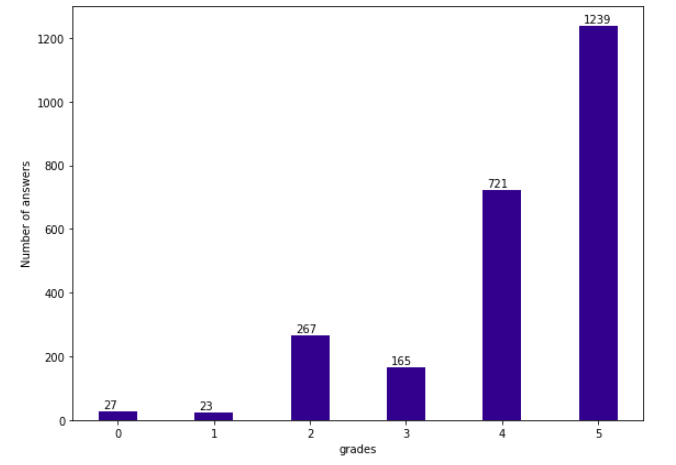
\includegraphics[scale=0.4]{images/mohler_multi_dist}
    	\caption{Multi-class distribution of Mohler'11 dataset.}
    	\label{mohler_multi_dist}
    \end{figure}
    
    
    
\end{document}
